\documentclass[11pt]{scrartcl}

\usepackage{ngerman}
\usepackage{fancyhdr}
\usepackage{cite}
\usepackage{pdfpages}
\usepackage{acronym}


\usepackage{array}
\usepackage{longtable}
\usepackage{booktabs}

\title{\documenttitle}
\subtitle{\documentsubtitle}
\author{Julian Rebholz,Tino Weber, Alex Jäger}
\date{\today}

\newcommand{\documenttitle}{6LoWPAN}
\newcommand{\documentsubtitle}{Einführung in die Technologie und Implementierung mit Contiki}

\pagestyle{fancy}
\fancyhf{}
\lhead{\documenttitle\ - Einführung und Implementierung}
\rhead{Verteilte Systeme}
\cfoot{\thepage}



\begin{document}
\maketitle
\newpage
\tableofcontents
\newpage
\input{einfuehrung.tex}
\newpage
\section{Der IEEE 802.15.4 Funkstandard}
IEEE 802.15.4 oder kurz 15.4 beschreibt einen Funkstandard, der bei geringer Datenrate die Leistungsaufnahme einzelner Teilnehmer möglichst weit zu reduzieren versucht. Das ist nötig, um den Anforderungen von Sensornetzwerken gerecht zu werden. \\
Durch den Standard werden der \ac{phy}- und \ac{mac}-Layer eines \ac{wpan} definiert. \\

\subsection{Teilnehmer und Topologien}
Dieses Kapitel deckt eigentlich Themen des Data Link Layers ab und ist im Kontext des entsprechenden Kapitels zu verstehen. Jedoch sind die Teilnehmer und Topologien des Netzwerks von so grundlegender Bedeutung, dass sie an dieser Stelle vorgezogen wurden. Alle Teilnehmer eines 15.4 \ac{pan} werden in zwei Kategorien eingeteilt:
\begin{itemize}
	\item Ein \ac{ffd} ist ein Teilnehmer mit vollständiger Implementierung von 15.4. Er kann alle Rollen annehmen.
	\item Ein \ac{rfd} hat reduzierte Fähigkeiten. Es kann nur mit einem FFD kommunizieren und somit nicht als Coordinator (siehe unten) auftreten.
\end{itemize}
15.4 ist gemäß IEEE für zwei verschiedene Netzwerk-Topologien ausgelegt:
\begin{itemize}
	\item Sterntopology
	\item Peer-to-Peer-Topology
\end{itemize}
\begin{figure}
	\centering
	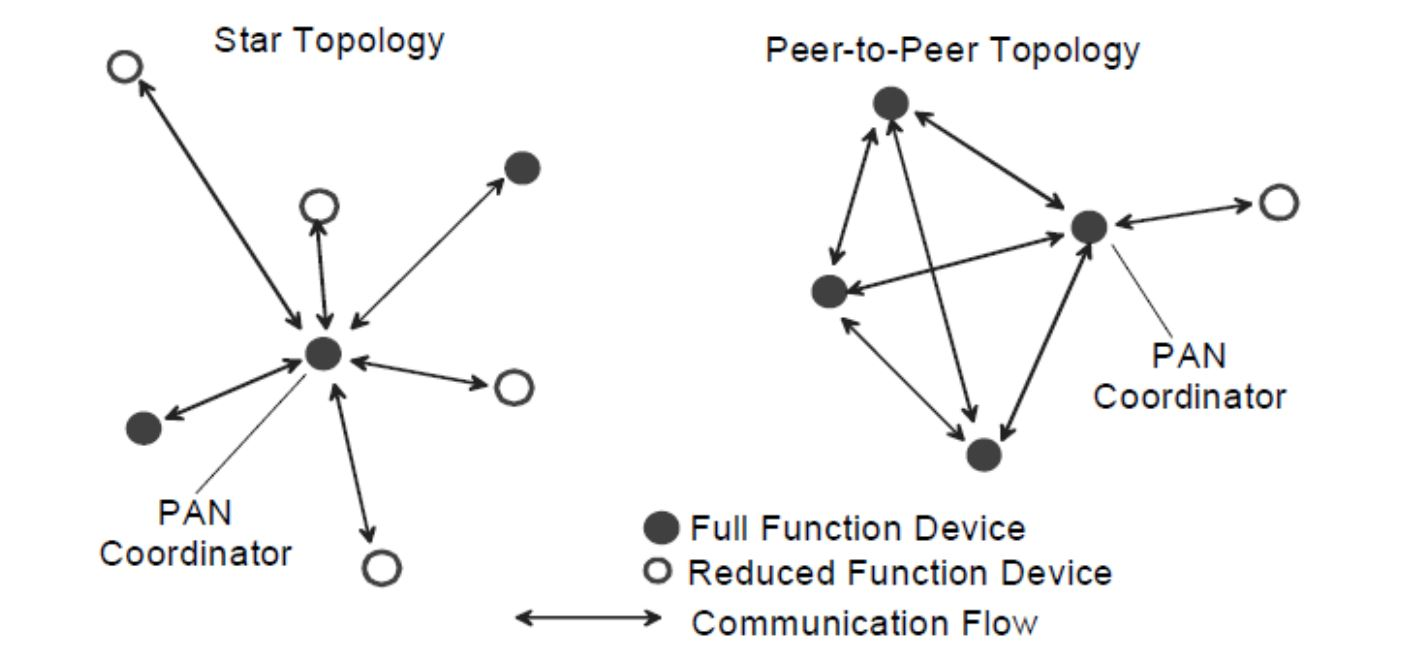
\includegraphics[width=0.7\textwidth]{Grafiken-Alex/topology.jpg}
	\caption{Topologien von 15.4-Netzwerken nach \cite[S.46]{ieee154}}
	\label{topology}
\end{figure}
In beiden Topologien existiert ein sogenannte \ac{pan}-Coordinator, der jedoch verschiedene Aufgaben übernimmt.\\
In einer Stern-Topologie ist der PAN-Coordinator der zentrale Kommunikationspunkt des Netzwerks. Alle Geräte kommunizieren nur mit ihm, was bedeutet, dass der Coordinator einen vergleichsweise hohen Energiebedarf hat. Die Teilnehmer hingegen müssen nur für ihre eigene Kommunikation aufwachen und können die restliche Zeit im Sleeping-Modus verbringen. Diese Topologie bietet sich an, wenn man einen netzbetriebenen Coordinator und mehrere batteriebetriebene Teilnehmer hat wie es z.B. in der Gebäudeautomatisierung oder bei \ac{pc} Peripheriegeräten der Fall ist.\\
Eine Peer-to-Peer-Topologie bietet sich offensichtlich für effizientes Routing an. Hierbei kommunizieren alle \ac{ffd} miteinander und \ac{rfd} als sogenannte Leafs mit einem \ac{ffd}. Anders als bei der Stern-Topologie ist somit der Coordinator nicht zentrale Kommunikationsstelle, sondern bietet Synchronisierungsservices o.ä. Diese Topologie bietet sich durch die Möglichkeit, Nachrichten per Multi-Hop zu routen im Bereich der Sensor-Netzwerke besonders an.\\
\begin{figure}
	\centering
	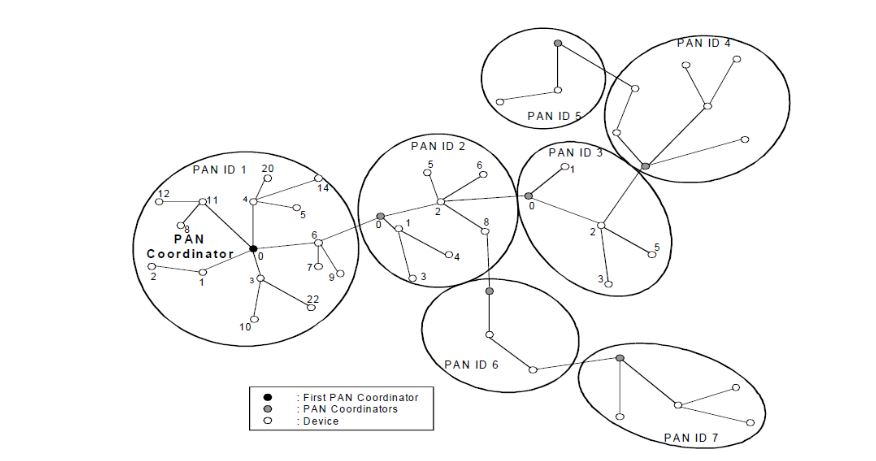
\includegraphics[width=\textwidth]{Grafiken-Alex/multicluster.jpg}
	\caption{Ein Multicluster Tree Netzwerk nach \cite[S.48]{ieee154}. Die Verbindungen zeigen nicht den Kommunikationsfluss, sondern Parent-Child-Beziehungen}
	\label{multicluster}
\end{figure}
Eine besondere Form der Peer-to-Peer-Technologie ist der Cluster Tree. Ein FFD beginnt einen neuen Cluster Tree, indem es eine freie PAN ID für das Netzwerk sucht und beginnt, sogenannte Beacons auszusenden. Das Device wird damit automatisch der Coordinator dieses Netzwerks. Ein Nachbar, der das Beacon empfängt, kann nun anfragen, am Netzwerk teilzunehmen. Erlaubt der Coordinator das, merkt er sich den Nachbarn als Child und dieser wiederum merkt sich den Coordinator als Parent. Der Nachbar beginnt nun seinerseits Beacons auszusenden, die weitere Geräte (auch solche, die nicht in direkter Reichweite des Coordinators sind) nutzen können, um dem Netzwerk teilzunehmen. Dadurch können große Netzwerke mit komplexen Routing-Tabellen entstehen. Darüber hinaus kann der PAN Coordinator einen Teilnehmer seines Netzwerks anweisen, ein eigenes Cluster zu konstruieren, bei dem er als PAN Coordinator auftritt. Dieser wiederum hält weiterhin Kontakt zu einem der Devices des originalen Netzwerks, wodurch große Multicluster-Netzwerke entstehen können. Grafik \ref{multicluster} zeigt ein solches Netzwerk. Durch diese Technik wird ein großer Netzwerkradius erreicht, wobei die Latenz einer Nachricht mit der Größe des Netzwerks zunimmt.\\

\subsection{Physical Layer}
\subsubsection{Genutzte Frequenzbänder}
15.4 nutzt die folgenden Frequenzbänder:
\begin{itemize}
	\item 2,4-2,4835 GHz ISM Band (16 Kanäle) weltweit
	\item 902-928 MHz ISM Band (10 Kanäle) in den USA
	\item 868-868,6 MHz Band (1 Kanal) in Europa
\end{itemize}
Dabei wird im 902MHz-Band ein Kanalabstand von 2 MHz und im 2,4GHz-Band ein Kanalabstand von 5 MHz eingesetzt. Die Kanäle werden mit Channel 0 (868 MHz), Channel 1-10 (902 MHz) und Channel 11-26 (2,4 GHz) bezeichnet.
\subsubsection{Genutzte Spreiz- und Modulationsverfahren}
Zum Verständnis der Modulation des Physical Layer durch 15.4 sind Kenntnisse über verschiedene Modulationsverfahren nötig. Diese sind im Folgenden kurz beschrieben. \\

\textbf{\ac{dsss}} \\
\begin{figure}
	\centering
	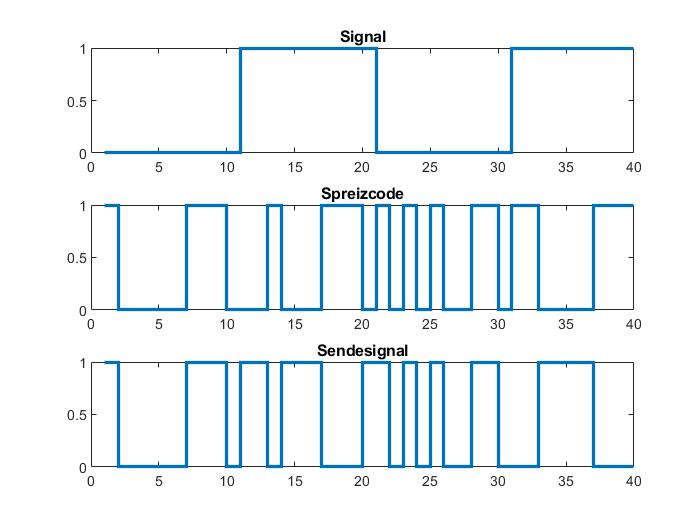
\includegraphics[width=0.7\textwidth]{Grafiken-Alex/dsss.jpg}
	\caption{Ein per DSSS gespreiztes Signal}
	\label{dsss}
\end{figure}
Das \acf{dsss} - ein sogenanntes Spreizverfahren - dient dazu, den Bitstrom auf ein breiteres Frequenzband zu spreizen. Dabei wird die ursprüngliche Bitfolge auf einen pseudo-zufällige Subbit-Strom moduliert. Die einzelnen Subbits dieses Stroms werden Chips genannt, der Strom Chipfolge oder Spreizcode.\\
In Abbildung \ref{dsss} wird das Signal mit einem Spreizcode unter Verwendung der XOR-Funktion gespreizt. Auf jedes Bit des Signals kommen dabei 10 Chips, wodurch eine Chiprate erreicht wird, die zehn Mal so hoch wie die Bitrate ist. Dieses Verhältnis wird auch Spreizfaktor genannt.\\
Sinn der DSSS ist es, ein Signal unempfindlicher schmalbandiger Störungen zu machen. Offensichtlich muss dem Empfänger zu Demodulation entweder der Spreizcode oder - da er pseudo-zufällig ist - der Generator zur Erstellung des Spreizcodes bekannt sein.\\

\textbf{\ac{bpsk}} \\
\begin{figure}
	\centering
	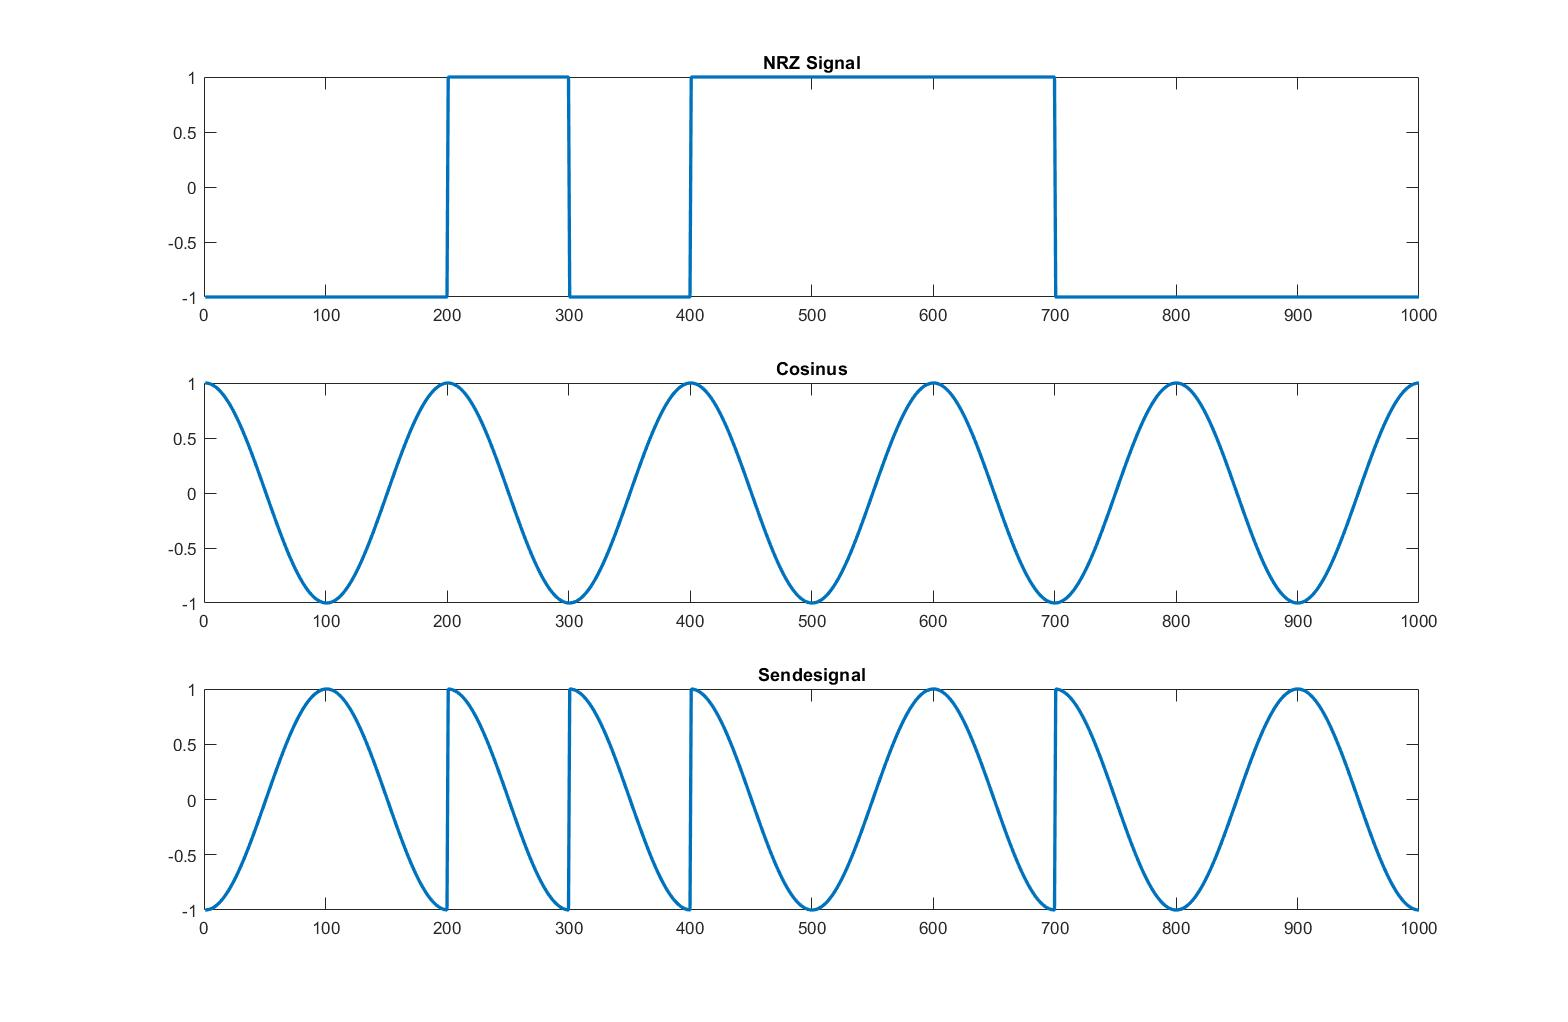
\includegraphics[width=0.7\textwidth]{Grafiken-Alex/bpsk.jpg}
	\caption{Ein BPSK-moduliertes Signal mit einer Cosinus-Schwingung als Träger}
	\label{bpsk}
\end{figure}
Die \acf{bpsk} ist die einfachste Form des Phase-Shift-Keyings. Die Bitfolge wird dabei als bipolares \ac{nrz} dargestellt und daraufhin mit dem Trägersignal multipliziert. Grafik \ref{bpsk} zeigt das Prinzip. \\

\textbf{\ac{oqpsk}}\\
\begin{figure}
	\centering
	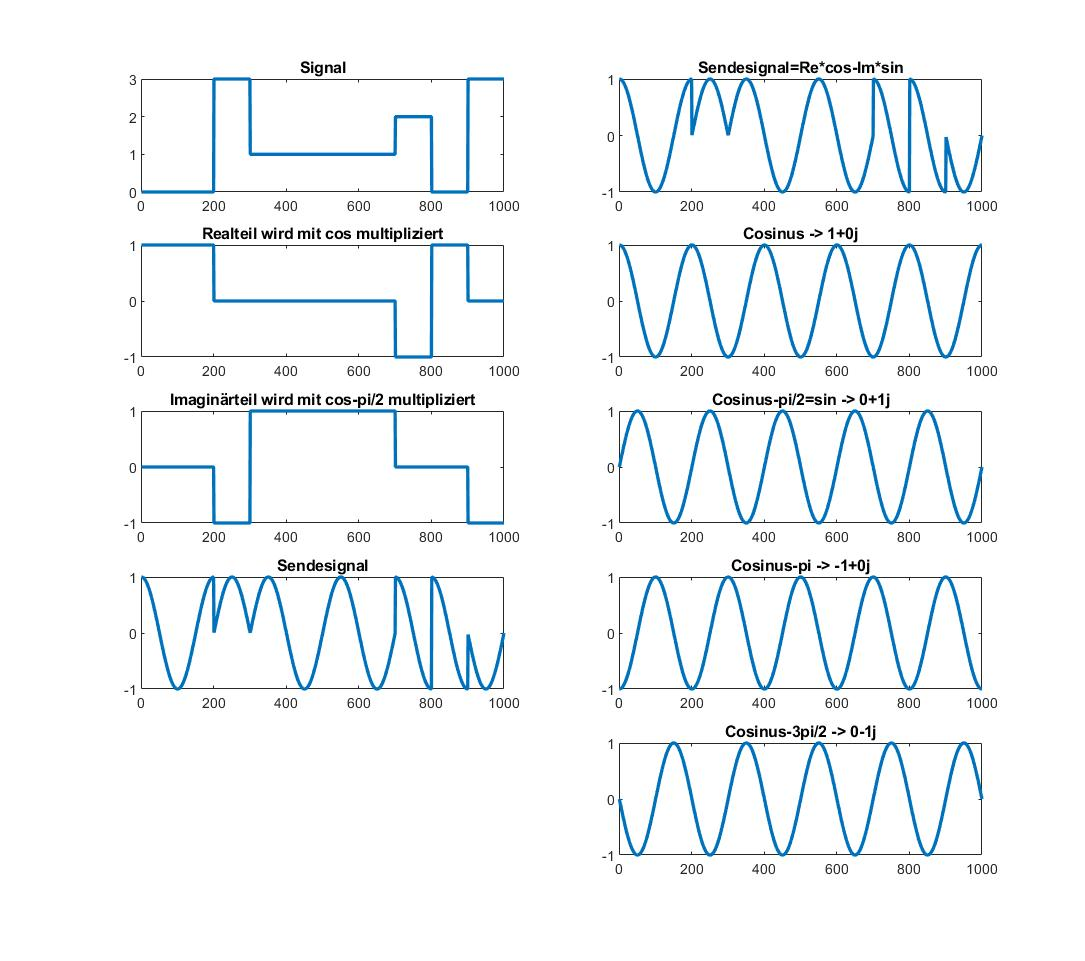
\includegraphics[width=\textwidth]{Grafiken-Alex/qpsk.jpg}
	\caption{Beispielhafte Erzeugung eines Sendesignals mit QPSK (links) und das Sendesignal im Vergleich mit phasenverschobenen Cosinus-Schwingungen (rechts).}
	\label{qpsk}
\end{figure}
Das \acf{oqpsk} ist eine komplexere Form des Phase-Shift-Keyings, bei der mit jedem Symbol ein Informationsgehalt von zwei Bits übertragen wird. Zunächst wird normales QPSK betrachtet. Hierbei wird der Bitstrom aufgeteilt in einen Real- und einen Imaginärbitstrom, wobei jedes zweite Bit in den Imaginärbitstrom fließt. Diese Ströme gehen daraufhin als Eingänge in einen \ac{qam} Modulator, welcher sie mit einem Cosinus (Real) bzw. Sinus (Imaginär) multipliziert und die Resultate subtrahiert, um das Sendesignal zu bilden.\\
Eine sinnvollere Aufteilung wird dadurch erreicht, dass der Bitstrom in der komplexen Zahlenebene so gemappt wird, dass der komplexe Zahlenstrom, der durch das Mapping entsteht gleichmäßig um den Ursprung verteilt ist. Das kann beispielsweise dadurch realisiert werden, dass die Zahlenfolge 00 als 0+0j dargestellt wird, die Zahlenfolge 01 als 0+1j usw. Häufig werden auch die resultierenden Werte um $\pi/4$ verschoben, also 00 auch 1+1j gemappt, 01 auf -1+1j usw.\\
Statt eines binären Zahlenstroms wird häufig ein Zahlenstrom mit Werten im Bereich [0,3] eingesetzt. Dieser hat die halbe Symbolrate des binären Stroms, aber statt einem zwei Bit/Symbol, wodurch wiederum die gleiche Bitrate erreicht wird. Der Vorteil besteht darin, dass er die gleiche Symbolrate wie der resultierende komplexe Zahlenstrom hat.\\
Die Erzeugung eines Signals mit QPSK ist in Grafik \ref{qpsk} anschaulich dargestellt.\\
Im Sendesignal ist klar erkennbar, dass bei Nulldurchgängen, also zum Beispiel von 1+0j zu -1+0j große Phasensprünge resultieren. Weil man dies vermeiden will, verschiebt man Real- und Imaginärteil des komplexen Signals um $\pi/2$ und bezeichnet das Resultat als Offset-QPSK oder kurz O-QPSK.\\

\subsubsection{Konkretes Modulationsverfahren}
\begin{figure}
	\centering
	
\includegraphics[width=\textwidth]{Grafiken-Alex/modulation.jpg}
	\caption{Ablauf der Modulation bei 15.4 aus \cite[S.412]{ieee154}}
	\label{modulation}
\end{figure}
Tatsächlich benutzt 15.4 eine Kombination aus DSSS und O-QPSK im 2,4GHz-Band und DSSS kombiniert mit BPSK in den restlichen Bändern. Der Ablauf der Modulationsverfahren ist in Abbildung \ref{modulation} dargestellt. Zunächst wird der Datenstrom in Oktette aufgeteilt. Jedes Oktett wird wiederum in zwei Symbole aufgeteilt, wobei die LSB (b0,b1,b2,b3) ein Symbol bilden und die MSB (b4,b5,b6,b7) ein anderes. Es ist darauf zu achten, dass das Symbol der LSB zuerst versendet wird.\\
Weil ein Symbol aus 4 bit besteht, kann es 16 verschiedene Werte annehmen. Entsprechend des Werts des Symbols wird einer von 16 verschiedenen, zueinander orthogonalen Spreizcodes verwendet, die im 2,4GHz-Band eine Länge von 32 Chips und in den restlichen Bändern eine Länge von 16 Chips haben und in der IEEE-Norm für das 2,4GHz-Band wie folgt festgelegt sind.\cite[S.413]{ieee154}\\
\begin{center}
	\begin{tabular}{cc}
		\textbf{Wert des Symbols} & \textbf{32-bit Spreizcode} \\
		0 &1 1 0 1 1 0 0 1 1 1 0 0 0 0 1 1 0 1 0 1 0 0 1 0 0 0 1 0 1 1 1 0\\
		1&1 1 1 0 1 1 0 1 1 0 0 1 1 1 0 0 0 0 1 1 0 1 0 1 0 0 1 0 0 0 1 0\\
		2&0 0 1 0 1 1 1 0 1 1 0 1 1 0 0 1 1 1 0 0 0 0 1 1 0 1 0 1 0 0 1 0\\
		3&0 0 1 0 0 0 1 0 1 1 1 0 1 1 0 1 1 0 0 1 1 1 0 0 0 0 1 1 0 1 0 1\\
		4&0 1 0 1 0 0 1 0 0 0 1 0 1 1 1 0 1 1 0 1 1 0 0 1 1 1 0 0 0 0 1 1\\
		5&0 0 1 1 0 1 0 1 0 0 1 0 0 0 1 0 1 1 1 0 1 1 0 1 1 0 0 1 1 1 0 0\\
		6&1 1 0 0 0 0 1 1 0 1 0 1 0 0 1 0 0 0 1 0 1 1 1 0 1 1 0 1 1 0 0 1\\
		7&1 0 0 1 1 1 0 0 0 0 1 1 0 1 0 1 0 0 1 0 0 0 1 0 1 1 1 0 1 1 0 1\\
		8&1 0 0 0 1 1 0 0 1 0 0 1 0 1 1 0 0 0 0 0 0 1 1 1 0 1 1 1 1 0 1 1\\
		9&1 0 1 1 1 0 0 0 1 1 0 0 1 0 0 1 0 1 1 0 0 0 0 0 0 1 1 1 0 1 1 1\\
		10&0 1 1 1 1 0 1 1 1 0 0 0 1 1 0 0 1 0 0 1 0 1 1 0 0 0 0 0 0 1 1 1\\11&0 1 1 1 0 1 1 1 1 0 1 1 1 0 0 0 1 1 0 0 1 0 0 1 0 1 1 0 0 0 0 0\\
		12&0 0 0 0 0 1 1 1 0 1 1 1 1 0 1 1 1 0 0 0 1 1 0 0 1 0 0 1 0 1 1 0\\
		13&0 1 1 0 0 0 0 0 0 1 1 1 0 1 1 1 1 0 1 1 1 0 0 0 1 1 0 0 1 0 0 1\\
		14&1 0 0 1 0 1 1 0 0 0 0 0 0 1 1 1 0 1 1 1 1 0 1 1 1 0 0 0 1 1 0 0\\
		15&1 1 0 0 1 0 0 1 0 1 1 0 0 0 0 0 0 1 1 1 0 1 1 1 1 0 1 1 1 0 0 0\\
	\end{tabular}
\end{center}

Für die restlichen Bänder werden die Symbole auf folgende Spreizcodes gemappt. \cite[S.414]{ieee154}
\begin{center}
	\begin{tabular}{cc}
		\textbf{Wert des Symbols} & \textbf{16-bit Spreizcode} \\
		0&0 0 1 1 1 1 1 0 0 0 1 0 0 1 0 1\\
		1&0 1 0 0 1 1 1 1 1 0 0 0 1 0 0 1\\
		2&0 1 0 1 0 0 1 1 1 1 1 0 0 0 1 0\\
		3&1 0 0 1 0 1 0 0 1 1 1 1 1 0 0 0\\
		4&0 0 1 0 0 1 0 1 0 0 1 1 1 1 1 0\\
		5&1 0 0 0 1 0 0 1 0 1 0 0 1 1 1 1\\
		6&1 1 1 0 0 0 1 0 0 1 0 1 0 0 1 1\\
		7&1 1 1 1 1 0 0 0 1 0 0 1 0 1 0 0\\
		8&0 1 1 0 1 0 1 1 0 1 1 1 0 0 0 0\\
		9&0 0 0 1 1 0 1 0 1 1 0 1 1 1 0 0\\
		10&0 0 0 0 0 1 1 0 1 0 1 1 0 1 1 1\\
		11&1 1 0 0 0 0 0 1 1 0 1 0 1 1 0 1\\
		12&0 1 1 1 0 0 0 0 0 1 1 0 1 0 1 1\\
		13&1 1 0 1 1 1 0 0 0 0 0 1 1 0 1 0\\
		14&1 0 1 1 0 1 1 1 0 0 0 0 0 1 1 0\\
		15&1 0 1 0 1 1 0 1 1 1 0 0 0 0 0 1\\
	\end{tabular}
\end{center}
\begin{figure}
	\centering
	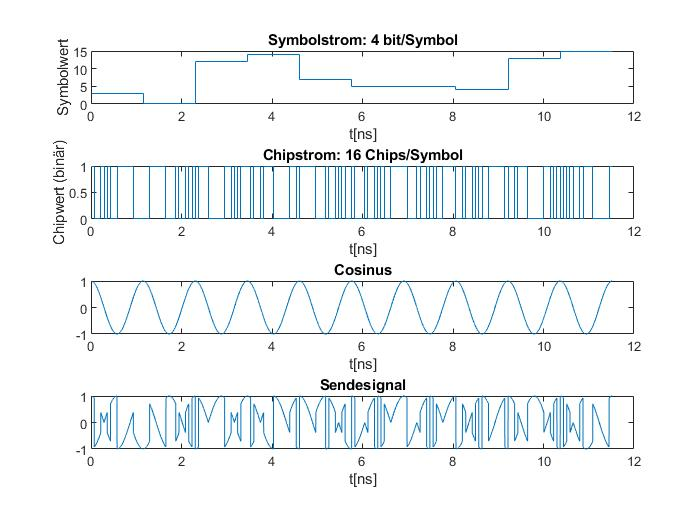
\includegraphics[width=\textwidth]{Grafiken-Alex/154modulation.jpg}
	\caption{Die vollständige Modulation eines Symbolstroms auf einen 868MHz-Träger unter Verwendung eines Alphabets mit 16 Chips/Symbol und BPSK als Modulationsart}
	\label{154modulation}
\end{figure}

Die so entstandenen Chipströme werden nun mit einem O-QPSK bzw. BPSK-Modulator moduliert. Zur Veranschaulichung zeigt Grafik \ref{154modulation} die gesamte Modulation eines Symbolstroms - dieser setzt sich aus 4 Bit/Symbol zusammen - zum analogen Sendesignal. \\

\subsection{Data Link Layer}
\begin{figure}
	\centering
	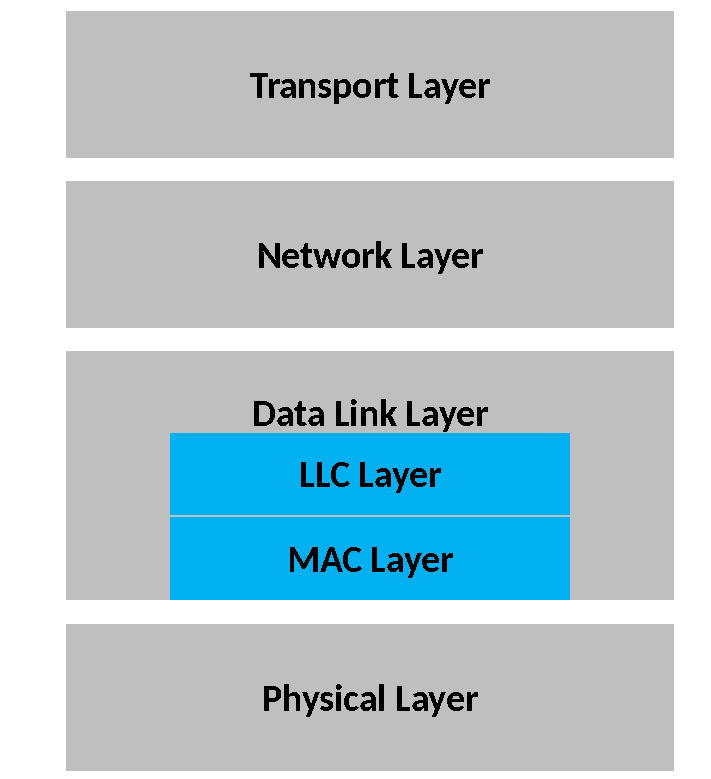
\includegraphics[width=0.5\textwidth]{Grafiken-Alex/ieee-osi.pdf}
	\caption{Die Unterteilung des Data Link Layers in LLC und MAC nach Norm des IEEE}
	\label{ieee-osi}
\end{figure}
Die IEEE unterteilt das aus dem OSI-Modell bekannte Data Link Layer in zwei Sublayer, die \ac{llc} Layer und \acf{mac} Layer heißen. Dabei ist der MAC-Layer in der Hirarchie unterhalb des LLC-Layers angesiedelt und wird häufig als Layer 2a, letzteres als Layer 2b bezeichnet. Grafik \ref{ieee-osi} zeigt die Aufteilung des Data Link Layers in LLC und MAC anschaulich.\\
Der LLC-Layer ist in IEEE 802.2 für alle Protokolle der 802-Norm definiert, hat sich aber in der Realität nicht durchgesetzt, weshalb der Network-Layer direkt auf den MAC-Layer zugreift. \cite{bartusch}IEEE 802.15.4 spezifiziert aus diesem Grund nur den MAC-Layer, weshalb im folgenden nicht auf die LLC-Schicht eingegangen wird. Die Begriffe Data Link Layer und Medium Access Layer können demnach im Kontext dieses Dokuments als Synonyme angesehen werden.
\subsubsection{MAC-Layer}
Wie bei vielen Funkübertragungstechniken üblich verwendet 15.4 den \ac{csmaca} Algorithmus. Ziel dabei ist es, Kollisionen auf dem Kanal zu vermeiden statt sie wie bei \ac{csmacd} zu erkennen und sich gegebenenfalls zurückzuziehen (z.B. per Arbitrierung). Die Nutzung von CSMA/CA bedeutet für einzelne Teilnehmer, dass sie zunächst auf dem Kanal lauschen müssen, um zu erkennen, ob dort gerade eine Kommunikation stattfindet und erst, wenn die Sendeleistung auf diesem Kanal einen bestimmten Wert unterschreitet - ergo es ist nur Rauschen vorhanden - senden darf. Abhängig vom genutzten Frequenzband kann er die verschiedenen zur Verfügung stehenden Kanäle analysieren und sich einen freien Kanal suchen (im 2,4-GHz-Band stehen immerhin 16 Kanäle zur Verfügung). \\

\textbf{MAC-Adresse}\\
Zur eindeutigen Identifizierung jedes Teilnehmers teilt sich jeder eine 8 Byte lange MAC-Adresse zu. Diese wird schon beim Flashen der Software festgelegt und bleibt somit über die Lebensdauer des Geräts bestehen. Die vollständige MAC-Adresse wird nach dem von der IEEE standardisierten Format \ac{eui64} erzeugt. Die ersten drei Bytes kennzeichnen demnach den Gerätehersteller, während die restlichen Bytes durch das Unternehmen selbst vergeben werden. Dadurch wird gewährleistet, dass jedes Gerät eine global einmalige MAC-Adresse erhält. \\
Weil eine 8 Byte lange MAC-Adresse offensichtlich gerade unter Berücksichtigung des gerade mal bis zu 127 Byte großen Frames eines 15.4 Pakets einen zu großen Overhead erzeugt - und die globale Einmaligkeit aufgrund der lokalen Beschränktheit eines Personal Area Networks ohnehin nicht relevant ist - kann der Teilnehmer sich bei der Anmeldung im Netzwerk durch den PAN Coordinator eine Kurzadresse (engl. Short Address) von zwei Bytes zuweisen lassen. Das beschränkt zwar die maximale Teilnehmerzahl eines Netzwerks auf 65535 Teilnehmer, jedoch sind Sensornetzwerke dieser Größenordnung ohnehin nicht realistisch. Im Jahr 2015 dürfte das größte Sensornetzwerk im Bereich von 1000 Sensorknoten gelegen haben. \cite{schiessleiot} \\

\textbf{Beacon und Non-Beacon Mode}\\
Im MAC-Layer gibt es zwei Möglichkeiten, den Kanalzugriff zu organisieren. Die einfachere davon ist der Non-Beacon Mode, bei dem die Teilnehmer durch simplen Einsatz des CSMA/CA Algorithmus wie oben beschrieben auf den Kanal zugreifen können. Das sorgt für eine sehr einfache Implementierung des MAC Layers, verzichtet aber auf die organisatorischen Vorteile des Beacon Modes.\\
Dieser setzt auf sogenannte Superframes. Ein Superframe ist ein Zeitrahmen, der mehrere Frames (=15.4 Pakete) überdauert. Ein Superframe wird durch das Aussenden eines Beacons durch den PAN Coordinator begonnen und endet mit dem Beginn des nächsten Superframes. Innerhalb eines Superframes lassen sich nun aktive Phasen und inaktive Phasen definieren, sodass den Teilnehmern des Netzwerks ermöglicht wird, zu gewissen Zeitpunkten in den Sleep-Modus zu gehen. Deshalb wird die inaktive Phase auch als Sleep Period bezeichnet.\\
\begin{figure}
	\centering
	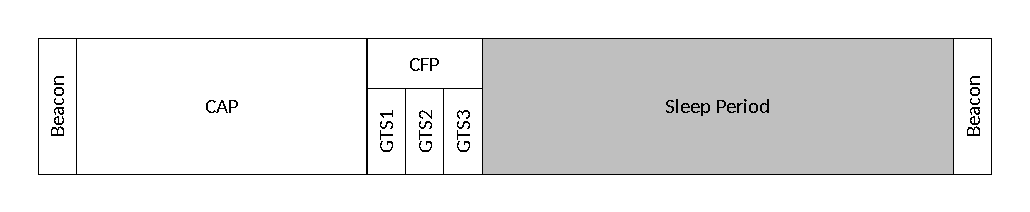
\includegraphics[width=\textwidth]{Grafiken-Alex/superframe.pdf}
	\caption{Inhalte eines Superframes bei Nutzung von 15.4 im Beacon Mode}
	\label{superframe}
\end{figure}
Die aktive Phase lässt sich weiter in \ac{cap} und \ac{cfp} unterteilen. \cite{superframestructure}. In ersterer ist der Kanal für alle Teilnehmer verfügbar und darf unter Verwendung des CSMA/CA-Algorithmus genutzt werden. Ein Teilnehmer - im Übrigen auch Node genannt - kann den Channel durch zweimaliges Aussenden des \ac{caa} Symbols reservieren und darf daraufhin seine Daten senden. \cite{sarodeslottedscmaca} Die CFP Periode wird in \ac{gts} unterteilt. Einem Teilnehmer kann also ein Slot zugewiesen werden, während dem er den garantierten alleinigen Zugriff auf den Kanal hat. Dabei ist anzunehmen, dass Nodes geringer Priorität ihre Daten während der CAP versenden und Nodes hoher Priorität eine GTS in der CFP zugewiesen bekommen. Nach Abschluss der CFP beginnt die Sleep Period. Die Länge der jeweiligen Perioden und ihre Existenz - CFP und Sleep Period sind optional - teilt der PAN Coordinator mit dem Inhalt des Beacons mit. Die ganze Struktur eines Superframes ist in Abbildung \ref{superframe} dargestellt. Es ist im Übrigen darauf zu achten, dass die CFP maximal sieben GTS bereitstellen darf.




\newpage
\section{6LoWPAN Adaption Layer und IPv6}
\newpage
	
	\section{Contiki als \ac{os} für verteilte Systeme}
	\subsection{\ac{6lowpan} Operating Systems im Vergleich}
	Es gibt mehrere  verschiedene Operating Systems, die einen \ac{6lowpan} Stack beinhalten. Diese Systeme unterstützen meistens die Protokolle, die in einem internetfähigen Gerät benötigt werden. Dadurch hat man ein System, welches die Kommunikation von der \ac{phy}- bis zur Application-Layer gewährleistet.\\
	Operating Systems, die diese Funktionalitäten bieten sind beispielsweise Contiki, TinyOS oder RIOT (Abb. \ref{os6lowpan}). All diese Operating Systems sind unter einer freien Lizenz verfügbar. Die Systeme werden innerhalb einer Github Repository entwickelt. Dies ermöglicht jedem User direkten Zugriff auf den gesamten Quellcode. TinyOS und Contiki sind mit einer BSD-Lizenz lizenziert. Dies bedeutet, dass der Programmierer, wenn er einen Binärcode veröffentlicht, nicht dazu verpflichtet ist auch den Quellcode zu veröffentlichen. Wird jedoch der nicht kompilierte Quellcode veröffentlicht, muss auch Die BSD-Lizenz im Quellcode vorhanden sein. RIOT hingegen ist mit einer GNU Lesser General Public License v2.1 lizensiert. Dies bedeutet, dass die Software in der eigenen Software verwendet und eingebunden werden kann, ohne dass der komplette Quellcode der darauf aufbauenden Software veröffentlicht werden muss. Werden jedoch Teile des lizenzierten Quellcodes verändert, so muss dieser Teil anderen Nutzern zugänglich gemacht werden.\\
	\begin{figure}
		\centering
		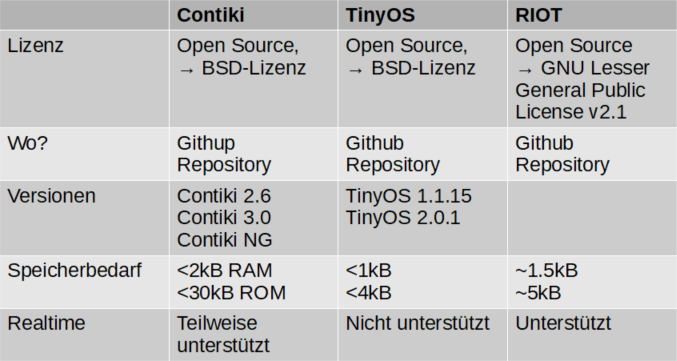
\includegraphics[scale=1]{Grafiken-Julian/OperatingSystemsVergleich.png}
		\caption{Operating Systems mit \ac{6lowpan} Implementierungen}
		\label{os6lowpan}
	\end{figure}
	Da \ac{6lowpan} auf ressourcensparenden Geräten zum Einsatz kommen soll, ist unter anderem auf den Energieverbrauch aber auch auf den Speicherbedarf zu achten. Contiki hat dabei den größten Speicherbedarf von ca. 2kB \ac{ram} und ca. 30kB \ac{rom}. Etwas weniger benötigt RIOT mit 1,5kB \ac{ram} und 5kB \ac{rom}. TinyOS ist in dieser Hinsicht führend mit ca. 1kB \ac{ram} und 4kB \ac{rom}. Nur RIOT ist wirklich Realtime fähig. Contiki unterstützt dies nur teilweise. TinyOS hingegen gar nicht. Da \ac{6lowpan} als Möglichkeit einer Realisierung von IOT gesehen wird, ist die Unterstützung von Realtime wichtig.\\
	Im Zuge der Recherche zu \ac{6lowpan} stellte sich heraus, dass diese Systeme alle noch in der Entwicklungsphase sind. Aufgrund mehrere Implementierungen eines \ac{6lowpan}-Netzwerkes mit Conitki, haben wir uns für dieses Operating System entschieden. Jedoch stellte sich auch hier im Laufe des Projekts heraus, dass die Dokumentation über dieses System und insbesondere auch den Quellcode sehr gering ist. Dies erschwerte die Nutzung des Systems erheblich.\\
	
	Contiki ist ein Open Source System, welches allgemein Low-Power Wireless Standarts unterstützt. Contiki besitzt die nötigen Stacks um mithilfe \ac{6lowpan} in einem Netz zu kommunizieren. Contiki unterstützt dabei verschiedene Protokolle in den verschiedenen Layern. Contiki unterstützt beispielsweise \ac{coap} aber auch \ac{http} im Application-Layer. Dadurch kann je nach Anwendung das passende Protokoll gewählt werden. Contiki unterstützt Protokolle wie \ac{ipv6}, \ac{udp}, \ac{tcp}, \ac{6lowpan} und viele weitere.\\
	Contiki selbst bezeichnet sich als „The Open Source Operating System for the Internet of Things“. Zielplattformen von Contiki sind batteriebetriebene Embedded Systems. Dadurch ergeben sich wichtige Anforderungen für das Betriebssystem:
	\begin{itemize}
		\item Speicher\\
		Ressourcenschonende Mikrocontroller besitzen nur wenig Speicher. Deshalb muss auch beim Betriebssystem darauf geachtet werden, dass möglichst wenig Speicher für das Betriebssystem selbst verbraucht wird. Dadurch soll genügend Speicher für die eigentlichen Anwendungsprogramme übrig bleiben.       
		\item Energieverbrauch\\
		\ac{6lowpan} sieht vor, dass ein Mikrocontroller-Knoten mehrere Jahre wartungsfrei von einer Batterie betrieben wird. Deshalb ist es sehr wichtig, dass das Betriebssystem Stromsparmaßnahmen vorsieht, damit solch lange Betriebszeiten mit einer Batterie realisiert werden können. Da \ac{6lowpan}-Knoten oft Sensoren sind, können deshalb nicht benötigte Peripherien des Mikrocontrollers des Sensors abgeschaltet werden. Als größter Energieverbraucher gilt jedoch das Funkmodul. Contiki besitzt deshalb ein System, welches das Funkmodul möglichst effizient an- bzw. ausschaltet.
	\end{itemize}
	
	Contiki ist deshalb auch nur für bestimmte Plattformen und Prozessoren verfügbar. Contiki unterstützt beispielsweise die MSP430x-Serie oder verschiedene AVR Mikrocontroller jeweils in Verbindung mit einem Funkmodul. Im vorliegenden Projekt wird das "'CC1310 Launchpad"' von Texas Instruments als Plattform verwendet. Im CC1310 Launchpad sind Prozessor und Funkmodul in einem Chip kombiniert, wodurch es möglich ist Contiki \ac{os} ohne zusätzlichen Peripherien(andere Boards) zu nutzen.
	
	\subsection{Protokollstacks}
	Contiki unterstützt den kompletten Protokollstack vom Physical Layer bis hin zum Application Layer. Contiki bietet dabei noch die Möglichkeit in den verschieden Layers verschiedene Protokolle zu verwenden. Dadurch kann Contiki viele verschiedene Einsatzgebiete haben, da je nach Anwendung das benötigte Protokoll ausgewählt werden kann. Abbildung \ref{protokollstack} zeigt dabei verschiedene Möglichkeiten den Protokollstack zu implementieren.\\
	\begin{figure}
		\centering
		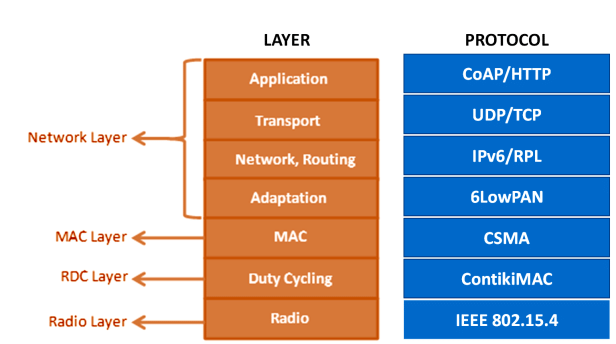
\includegraphics[scale=0.5]{Grafiken-Julian/ProtokollStacksContiki.png}
		\caption{Protkollstack des Contiki Operating Systems, \cite{contikiprotokollstack}}
		\label{protokollstack}
	\end{figure}
	Auf den unteren Layern (\ac{phy}) teilt sich der Stack von Contiki in zwei Layer auf. Zum einen in den \ac{15.4} Stack und den ContikiMAC Stack, der zwischen \ac{phy}- und \ac{mac}-Layer liegt. Der ContikiMAC Layer nimmt dabei eine ganz besondere Funktion ein. Der ContikiMAC ist unter anderem dafür verantwortlich, dass das Funkmodul möglichst wenig aktiv ist. Das Funkmodul ist im gesamten System der größte Energieverbraucher und wird deshalb nur sequenziell an und ausgeschaltet. Abbildung \ref{ContikiMAC} zeigt die verschiedenen Möglichkeiten wie ein Paket mit und ohne Phasenoptimierung verschickt beziehungsweise empfangen werden kann. Im Falle ohne Phasen-Optimierung, sendet der Sender so lange (mit der Bedingung, dass das der Sendezeitraum nicht eingeschränkt ist), bis der Sender ein \ac{ack}-Paket vom Empfänger erhält. Der Energieverbrauch ist in diesem Fall unnötig hoch, da ein Node so programmiert ist, dass er nur in bestimmten Zeitabschnitten eine Funkkommunikation aufbaut. Der Sender kann deshalb, ausgehend von früheren Kommunikationen zum Node speichern, wann ein Node zur Kommunikation bereit ist. Durch dieses Verfahren wird der Energieverbrauch erheblich gesenkt. Der ContikiMAC trägt damit hauptsächlich dazu bei, dass der Stromverbrauch der Nodes gering gehalten werden kann. Der \ac{mac} Layer in Contiki benutzt auch \ac{csmaca}. Dadurch wird sichergestellt, dass mehrere Nodes nicht gleichzeitig senden und Pakete über Funk korrekt empfangen werden. \\
	\begin{figure}
		\centering
		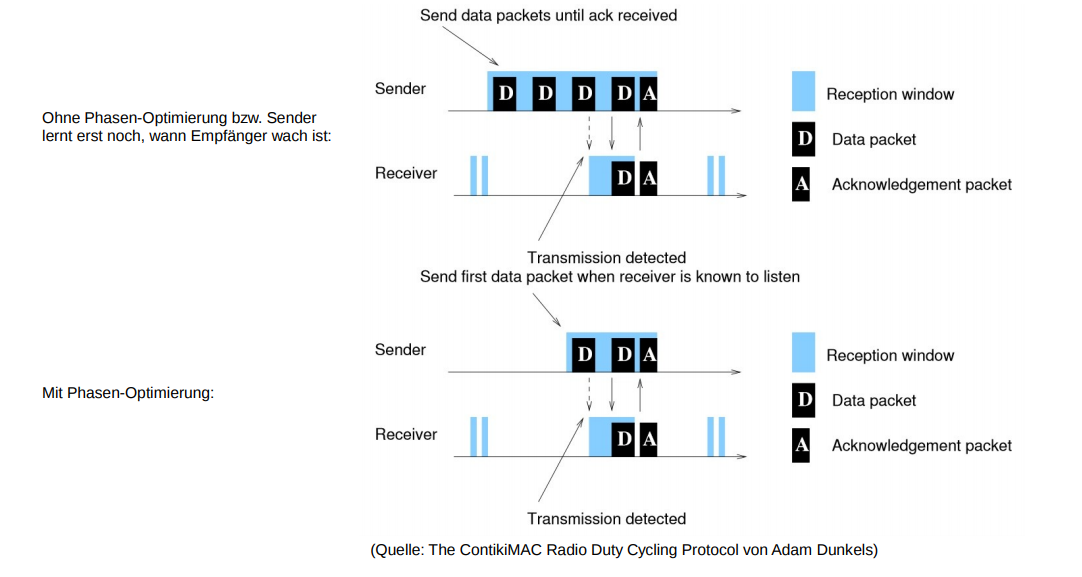
\includegraphics[scale=0.5]{Grafiken-Julian/ContikiMAC.png}
		\caption{Funktionsweise des ContikiMAC's mit Phasenoptimierung, \cite{dunkelsmac}}
		\label{ContikiMAC}
	\end{figure}
	Nach dem \ac{csmaca} Stack folgt der \ac{6lowpan} Stack, der als Adaptionslayer zwischen \ac{ipv6} und und dem \ac{mac}-Layer dient. Mithilfe des \ac{6lowpan} Protokoll wird der Header der überliegenden Layern erheblich verkleinert. Durch das \ac{6lowpan} Protokoll kann der Header eines \ac{ipv6} Pakets so verkleinert werden, dass die maximal zulässige Größe eines \ac{15.4} Pakets eingehalten werden kann. Deshalb ermöglicht dieses Protokoll erst die Nutzung des \ac{15.4} Protokolls und damit eine energiesparende Funkübertragung.\\
	Im Network Layer bietet Contiki die Nutzung von \ac{ipv6} und \ac{rpl}. \ac{rpl} baut das Kommunikationsnetz mit zielgerichteten Graphen auf. Dabei unterscheidet man zwischen \ac{dag} und \ac{dodag}. Ein \ac{dag}-Graph hat dabei mehrere Zielknoten jedoch nur eine Linie (ohne Schleifen zum Zielknoten). Ein \ac{dodag}-Graph hingegen hat nur einen Zielknoten aber dafür gibt es mehrere Wege zum Zielknoten(vgl. Abbildung \ref{RPL_DAG_DODAG}).\\
	\begin{figure}
		\centering
		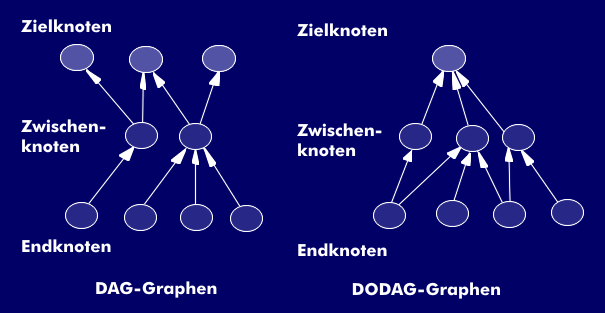
\includegraphics[scale=0.5]{Grafiken-Julian/RPL_DAG_DODAG.png}
		\caption{verschiedene Graphentypen beim RPL, \cite{rpldagdodag}}
		\label{RPL_DAG_DODAG}
	\end{figure}
	Auf der Transportschicht kann man sich für \ac{tcp} oder \ac{udp} entscheiden. \ac{tcp} macht jedoch in Kombination mit \ac{6lowpan} und \ac{15.4} wenig Sinn, da \ac{tcp} einen noch größeren Header besitzt als \ac{udp}. Da \ac{tcp} nicht komprimiert wird, ist dies allein aufgrund der Headergröße nicht möglich. \ac{tcp} ist ein verbindungsorientiertes Protokoll und bietet deshalb mehr Sicherheit, dass Pakete richtig (in der richtigen Reihenfolge, keine Bitfehler...) empfangen werden. Da mit \ac{6lowpan} ein Sensornetzwerk betrieben werden soll, wo die Sensoren beispielsweise nur jede Minute einen neuen Wert liefern, kann es auch vernachlässigt werden, wenn einzelne Nachrichten falsch oder gar nicht ankommen. Da \ac{udp} auf bestimmte Sachen aus dem \ac{tcp} Protokoll verzichtet, wird es allgemein als das unkompliziertere und schnellere Verbindung angesehen.\\
	Auf der Applikationsschicht kann zwischen \ac{coap} und \ac{http} entschieden werden. Wie bei \ac{tcp} und \ac{udp}, ist \ac{coap} im Vergleich zu \ac{http} das schlankere Protokoll und bietet sich deshalb auch für ein \ac{6lowpan} Netzwerk an.\\
	
	Contiki \ac{os} hat den Vorteil, dass es viele Protokollstacks beinhaltet. Dadurch kann individuell an die benötigten Strukturen der Anwendung der Stack "'zusammengesucht"' werden. Hauptgebiet von Contiki \ac{os} bleiben jedoch vorerst \ac{6lowpan} Netzwerke.
	
	\subsection{Prozess}
	Contiki \ac{os} basiert auf verschiedenen Prozessen. Diese Prozesse werden eventbasiert aufgerufen. In Contiki gibt es grundsäzlich zwei verschiedene Arten wie ein Prozess ausgeführt werden kann.
	\begin{itemize}
		\item Kooperativ\\
		Kooperative Prozessen werden nacheinander aufgerufen. Sobald ein Prozess beendet wurde, kann der nächste Prozess gestartet werden. Der Aufbau der Prozesse darf jedoch nicht direkt mit einem RTOS verglichen werden, da ein Prozess nicht sequentiell aufgerufen wird, sondern nur dann wenn dieser Prozess auch ausgelöst (Event) wurde. Ein kooperativer Prozess unterbricht nie einen laufenden Prozess. Kooperative Prozessen sind Bestandteil der ganz normalen Programmausführung.
		\item Präventiv\\
		Ein präventiver Prozess ist vergleichbar mit einem Interrupt. Ein präventiver Prozess unterbricht den laufenden Prozess und wird dann ausgeführt. Nach Beenden des präventiven Prozesses springt das \ac{os} in den unterbrochenen Prozess zurück. Dieser kann anschließend fortgeführt werden. 
	\end{itemize}
	
	Contiki \ac{os} ist grundsätzlich so aufgebaut, dass es viele kooperative Prozesse gibt und nur einzelne präventive Prozesse, die den "'normalen"' Programmablauf unterbrechen. Der Programmablauf wird mithilfe einer Eventqueue im Kernel geregelt. Die Eventqueue wird nach dem Prinzip eines \ac{fifo} abgearbeitet. Ist die Eventqueue leer werden deshalb auch so lange keine Prozesse mehr ausgeführt bis ein neuer Event in die Eventqueue geschrieben wird.
	
	Den Quellcode, wie ein Prozess deklariert wird, zeigt Abbildung \ref{ContikiProzess}. Der Name des Prozesses wird mit PROCESS\_THREAD("'Prozessname"') festgelegt. Der eigentliche Prozess wird dann innerhalb PROCESS\_BEGIN() und PROCESS\_END() definiert. PROCESS\_BEGIN(), PROCESS\_END() und PROCESS\_THREAD() sind lediglich Defines, die die Programmierung von Prozessen vereinfachen soll. Die Defines stellen dabei in Kombination eine Switch Case Abfrage dar. Mithilfe dieser Struktur wird der ganze Prozessablauf in Contiki \ac{os} geregelt.
	\begin{figure}
		\centering
		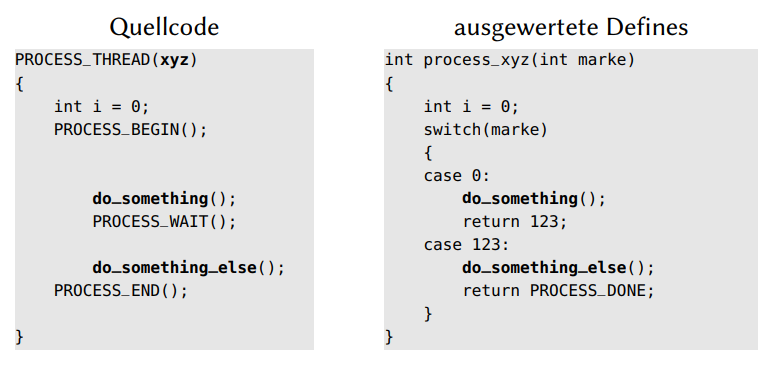
\includegraphics[scale=0.5]{Grafiken-Julian/Contiki_Prozess.png}
		\caption{Aufbau eines Contiki-Prozess, \cite[S.9]{ausgewertetedefines}}
		\label{ContikiProzess}
	\end{figure}
	Diese Defines, die den Code vereinfachen sollen bezeichnet man in Contiki als Protothreads. Um einen Prozess zu strukturieren bietet Contiki \ac{os} mehrere solcher Protothreads an. Die in Contiki \ac{os} vorhanden Protothreads sind:
	
	\begin{itemize}
		\item PROCESS\_BEGIN()\\
		Mit PROCESS\_BEGIN wird der Anfang eines Prozesses deklariert. Der eigentliche Code des Prozesses startet nach PROCESS\_BEGIN().
		\item PROCESS\_END\\
		Mit PROCESS\_END() wird das Ende eines Prozesses deklariert. PROCESS\_BEGIN() und PROCESS\_END() müssen in jedem Przess angegeben sein. Diese beiden Defines deklarieren den Programmcode des Prozesses.
		\item PROCESS\_EXIT()\\
		Mit PROCESS\_EXIT() wird ein der Prozess verlassen. Der Unterschied zwischen PROCESS\_END() und PROCESS\_EXIT() liegt darin, dass das Define PROCESS\_END() in jeder Prozessdeklarierung enthalten sein muss. PROCESS\_EXIT() kann dann zum Beispiel in einem Unterpfad verwendet werden um den Prozess zu beenden.
		\item PROCESS\_WAIT\_EVENT\\
		Mit PROCESS\_WAIT\_EVENT wird der Prozess solange pausiert, bis irgendein Event auftritt. Während der Prozess auf einen Event wartet, können andere Prozesse ausgeführt werden. Allerdings löst dieser Event den Prozess erst aus, wenn der auslösende Event durch die Eventqueue zum Kernel gelangt ist.
		\item PROCESS\_YIELD()\\
		Mit PROCESS\_YIELD() wird wie bei PROCESS\_WAIT\_EVENT() der Prozess solange pausiert bis ein Event auftritt.
		\item PROCESS\_WAIT\_EVENT\_UNTIL()\\
		Mit PROCESS\_WAIT\_EVENT\_UNTIL() wird der Prozess nur ausgeführt, wenn ein bestimmter Event ausgelöst wurde. Der nachfolgende Code wird also nur unter bestimmten Eventbedingungen ausgeführt.
		\item PROCESS\_WAIT\_UNTIL()\\
		Mit PROCESS\_WAIT\_UNTIL() wird auf irgendeine Bedingung gewartet. Allerdings besteht bei diesem Protothread die Möglichkeit, dass der Prozess nicht abgegeben wird. Der Prozess befindet sich dann möglicherweise in einer Endlosschleife und das Programm wird nicht weiter ausgeführt.
		\item PROCESS\_PAUSE()\\
		Mit PROCESS\_PAUSE() wird der Prozess kurz pausiert und eine andere Prozess kann ausgeführt werden.
	\end{itemize}
	Protothreads die auf einen Event warten, bis dieser ausgelöst wurde, bieten die Möglichkeit den Programmablauf gut zu strukturieren. Wichtig ist dabei, dass andere Prozesse ausgeführt werden können während ein anderer Prozess auf einen Event wartet.
	
	\subsection{Events}
	Contiki \ac{os} ist ein eventbasiertes Betriebssystem. Events nehmen bei Contiki deshalb eine wichtige Rolle ein. Ohne Events wird der Programmcode von Contiki nur einmal ausgeführt. Erst durch Events wird der Programmcode flexibel. Contiki \ac{os} besitzt deshalb drei verschiedene Arten von Events:
	
	\subsubsection{Asynchroner Event}
	Ein asynchroner Event wird durch den Aufruf von process\_post() aufgerufen. Parameter die dabei übergeben werden müssen, sind der Pointer zum Prozess, welcher Event Identifier ausgelöst werden soll und eine optionale Nachricht, die mitgesendet werden kann. In der Nachricht werden hauptsächlich Daten mitübertragen, die ausgewertet oder bearbeitet werden sollen. Abbildung \ref{BeispielProgramm} zeigt ein Beispielcode, wie ein Event angelegt und ausgelöst werden kann. Außerdem wird ein PROCESS\_EVENT\_TIMER Event abgearbeitet.\\
	Ein asynchroner Event wird nicht sofort ausgeführt wenn er ausgelöst wurde. Mit process\_post() wird der Event in eine Eventqueue hineingeschrieben. Diese Eventqueue wird vom Kernel abgearbeitet. Die Eventqueue wird nach dem Prinzip eines \ac{fifo}s abgearbeitet. 
	
	\begin{figure}
		\centering
		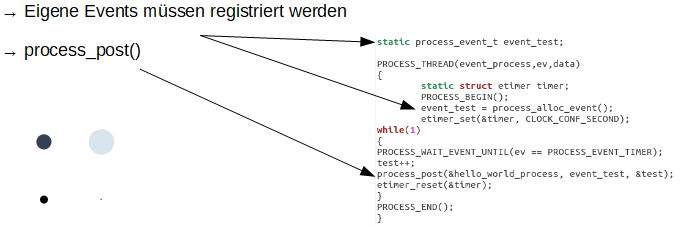
\includegraphics[scale=0.8]{Grafiken-Julian/ContikiEventsCodebeispiel.png}
		\caption{Beispielprogramm mit auslösen eines Events}
		\label{BeispielProgramm}
	\end{figure}
	
	\subsubsection{Synchroner Event}
	Ein synchroner Event ist vergleichbar mit einem Funktionsaufruf in C. Bei diesem Event wird der Prozess innerhalb des anderen Prozesses aufgerufen. Der aufrufende Prozess ist dann eine Ebene über dem aufgerufenen Prozess. Nachdem der aufgerufene Prozess beendet wurde wird der ursprüngliche Prozess weiter ausgeführt. Eine solcher Event wird mit process\_post\_synch() ausgelöst. Wie bei einem asynchronen Prozess werden der Funktion die Parameter des Pointer der Funktion die aufgerufen werden soll, welcher Event Identifier ausgelöst wird und eine Nachricht übergeben. Der aufgerufen Prozess kann dabei jedoch nicht unterscheiden, ob er von einem asynchronen oder einem synchronen Event ausgelöst wurde.
	\subsubsection{Polling Event}
	Ein poll Event entspricht einem normalen Interrupt. Das heißt, der Event wird sofort ausgeführt. Der laufende Prozess wird dann unterbrochen und die Pollingroutine wird ausgeführt. Diese Event-Funktion ist dann wichtig, wenn zeitkritische Aufgaben (Bsp: Empfang Daten) ausgeführt werden müssen. Ein poll Event wird mit der Funktion process\_poll() ausgelöst. Im Unterschied zu asynchronem und synchronem Event wird lediglich der Prozess anhand seines Pointers aufgerufen. Es wird kein spezieller Event Identifier ausgelöst und es werden keine Nachrichten übermittelt.\\
	
	Alle Arten von Events werden bei Contiki \ac{os} öfters genutzt. Der Programmablauf wird hauptsächlich mit asynchronen Events geregelt. Deshalb nehmen diese Events eine besondere Stellung bei Contiki ein. Abbildung \ref{EventsContiki} zeigt Quellcode, wie die verschiedenen Arten von Events ausgelöst werden können.\\
	Conitiki \ac{os} bietet dem Programmierer 127 frei nutzbare Event Identifiers an. Der Programmierer hat dadurch die Möglichkeit eigne Events zu erstellen, die in seinem Programm gebraucht werden. Contiki hat darüber hinaus acht für den Kernel reservierte Event Identifier:
	\begin{itemize}
		\item PROCESS\_EVENT\_INIT\\
		Dieser Event Identifier wird dem Prozess bei Start von Contiki \ac{os} gesendet
		\item PROCESS\_EVENT\_POLL\\
		Dieser Event Identifier erhält ein Prozess der mit einem poll Event asugelöst wurde.
		\item PROCESS\_EVENT\_EXIT\\
		Diesr Event Identifier wird an einem Prozess gesendet, der vom Kernel beendet wurde. Anschließend wird der vom Prozess benötigte Speicherbereich wieder freigegeben.
		\item PROCESS\_EVENT\_CONTINUE\\
		Diesen Event Identifier erhält ein Prozess, der in einer PROCESS\_YIELD() Operation wartet. Anschließend wird der Prozess weiter ausgeführt.
		\item PROCESS\_EVENT\_MSG\\
		Dieser Event Identifier wird einem Prozess gesendet, wenn eine Kommunikations-Nachricht empfangen wurde. Typischerweise verwendet der IP Stack diesen Identifier um einen anderen Prozess zu informieren, dass eine Nachricht empfangen wurde.
		\item PROCESS\_EVENT\_EXITED\\
		Dieser Identifier wird an alle Prozesse gesendet. Der Event Identifier tritt auf, wenn ein Prozess beendet wurde. Der Kernel informiert damit die übrigen Prozesse, dass ein bestimmter Prozess nicht mehr existiert. Die übrigen Prozesse können dann durch den beendeten Prozess belegten Speicher im eigenen Prozess wieder freigeben.
		\item PROCESS\_EVENT\_TIMER\\
		Dieser Identifier wird ausgelöst, wenn ein Eventtimer (etimer) abgelaufen ist.
	\end{itemize}	
	Die genannten Event Identifiers werden hauptsächlich für die interne Regelung von Prozessen genutzt. Ein üblicher Programmierer kommt hauptsächlich mit dem PROCESS\_EVENT\_TIMER Event in Kontakt. Die anderen Kernel-Events werden vom Kernel unbemerkt erzeugt und  von den Prozessen verarbeitet, sodass der Programmierer dies nicht bemerkt.
	
	\subsection{Prozess Scheduler}
	Der Prozess Scheduler in Contiki regelt den gesamten Programmablauf. Er ist dafür verantwortlich, dass alle Events den richtigen Prozess erreichen. Dabei sorgt er auch dafür, dass der Datenfluss, der mit einem Event einhergeht reibungslos verläuft. Der Prozess Scheduler ist auch welcher, der das komplette Programm startet.\\ 
	Um ein Programm zu starten, ruft er die Funktion process\_start() auf. Diese Funktion sendet an den aufgerufenem Prozess den PROCESS\_EVENT\_INIT Event Identifier. Daraufhin startet der Prozess(vgl. Abbildung \ref{EventsContiki}). In Contiki selbst wird dies oft direkt bei der Initialisierung gemacht. Der Aufruf lautet dabei AUTOSTART\_PROCESS(), wobei die Parameter der Funktion die einzelnen Adresspointer auf die einzelnen Prozesse sind. Üblicherweise beendet sich der Prozess irgendwann wieder von selbst mit PROCESS\_EXIT() oder PROCESS\_END(). Allerdings besitzt der Prozess Scheduler die Möglichkeit einen Prozess mit proccess\_exit() von außen zu beenden. Dann werden wiederum die belegten Ressourcen des Prozesses freigegeben. Der Prozess Scheduler ist dabei auch jener, der die anderen Prozesse informiert, dass ein anderer Prozess beendet wurde.
	\begin{figure}
		\centering
		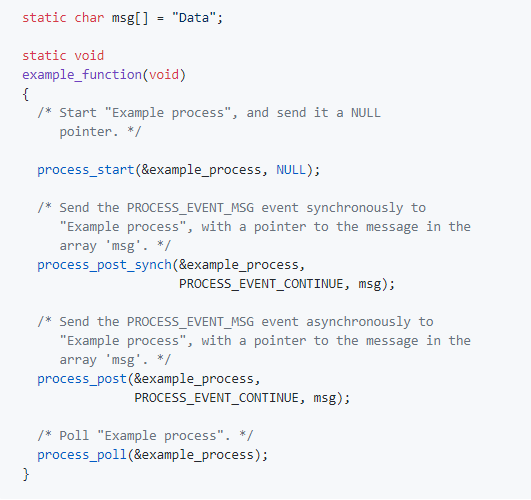
\includegraphics[scale=0.5]{Grafiken-Julian/ContikiEvents.png}
		\caption{Codebeispiel: Auslösen verschiedener Eventarten in Contiki \ac{os}, \cite{codebesipiel}}
		\label{EventsContiki}
	\end{figure}
	\subsection{Contiki Makefile und kompilieren eines Projekts}
	Um ein Contiki \ac{os} Projekt kompilieren zu können, müssen im Projektordner mit dem Programmcode noch weitere Files vorliegen. Ohne das Makefile wird der Programmcode nicht kompiliert. Im Makefile stehen Information für den Compiler bezüglich Projektname, wo Headerdateien zu finden sind und optionale  Defines, um Code flexibel einbinden zu können oder auszuschließen. Ein weiteres wichtiges File ist das Makefile.target, welches ebenfalls optional ist. Wird das Makefile.target nicht erstellt, muss das Target dann dem Compiler vor dem kompilieren angegeben werden. In Instant Contiki wird das Kompilieren mit dem Terminal erledigt. Ein beispielhafter Befehl, wie ein Programm kompiliert werden kann, zeigt Abbildung \ref{Makefile&Kompilieren}. \\
	Contiki \ac{os} ist so gestaltet, dass es für verschiedene Plattformen (Prozessoren,Boards) bereits fertige Implementierungen gibt. Deshalb muss immer eine Target angegeben werden. Das hier vorliegende Beispiel soll für das CC1310 Launchpad von Texas Instruments kompiliert werden. Das Target ist deshalb "'srf06-cc26xx"' und das benutzte Board ist das CC1310 Launchpad von Texas Instruments. hello-world.bin in Abbildung \ref{Makefile&Kompilieren} steht dafür, dass der Programmcode in Binärdateien kompiliert werden soll.
	\begin{figure}
		\centering
		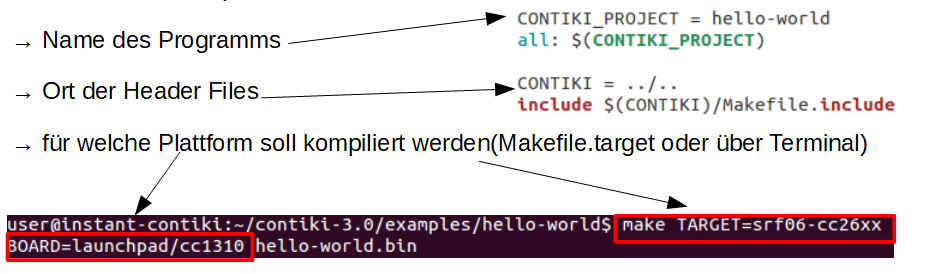
\includegraphics[scale=0.5]{Grafiken-Julian/MakefileKompilieren.png}
		\caption{Erzeugen von Binärdateien mithilfe des Terminals in Instant Contiki}
		\label{Makefile&Kompilieren}
	\end{figure}
	\subsubsection{CC1310 Launchpad und dessen Konfigurationsdateien in Contiki \ac{os}}
	Contiki \ac{os} besitzt für eine Plattform bereits vordefiniert, welche Schnittstellen das Board oder der Prozessor besitzt. Diese Definitionen werden beim Kompilieren eines Projektes verwendet. Die Prozessor spezifischen Einstellungen befinden sich dabei im Conitki-conf.h File. In Contiki-conf.h wird beispielsweise definiert mit welcher Baudrate eine UART-Schnittstelle arbeitet oder bezogen auf \ac{6lowpan}, welche Kompressionsmethode und ab welcher Payload eine Fragmentierung der Pakete vorgenommen werden soll (vgl. Abbildung \ref{Contiki-conf}).\\
	\begin{figure}
		\centering
		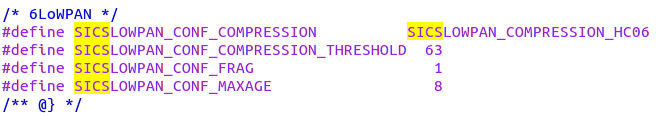
\includegraphics[scale=0.5]{Grafiken-Julian/Contiki_conf.png}
		\caption{Codeauszug des Contiki-conf.h File der srf06-cc26xx Plattform}
		\label{Contiki-conf}
	\end{figure}
	Das board.h File beinhaltet Definitionen bezüglich Pinbelegung (bsp: Pins die an einen Button angeschlossen sind). Contiki hat dabei bereits vordefinierte Defines für Button, sodass der Programmierer theoretisch nicht mal wissen muss, an welchen Pin ein Button oder eine Peripherie angeschlossen ist. Abbildung \ref{Boardfiles} zeigt beispielhaft einen Codeauszug aus dem board.h File des CC1310 Launchpads. Die Buttons werden hier dem Pin zugeordnet. Dadurch kann Code leicht auf andere Boards importiert werden ohne den kompletten Code an die neue Plattform anpassen zu müssen. Contiki \ac{os} ist deshalb sehr flexibel für verschieden Plattformen einsetzbar.\\
	\begin{figure}
		\centering
		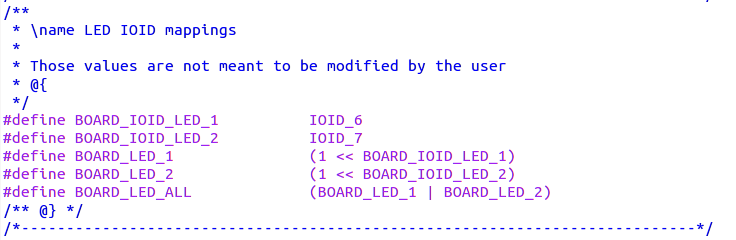
\includegraphics[scale=0.5]{Grafiken-Julian/Boardfiles.png}
		\caption{Codeauszug des board.h File des CC1310 Launchpad in Contiki}
		\label{Boardfiles}
	\end{figure}
	Das in diesem Projekt verwendete Board ist das CC1310 Launchpad. Das Launchpad kann direkt als Funkmodul verwendet werden, da eine PCB Antenne auf dem Launchpad angebracht ist. Außerdem besitzt es zwei Buttons, die als externe Interrupts verwendet werden können. Das CC1310 Launchpad hat den CC1310 Mikrocontroller verbaut. Dieser besteht aus zwei verschiedenen Prozessoren. Zum einen aus eine ARM Cortex-M3 und einem ARM Cortex-M0. Der ARM Cortex-M3 ist die Haupt-CPU. An ihm sind die ganzen Peripherien (UART, I2C, Timer...) angeschlossen. Der ARM Cortex-M3 regelt die nicht funkbasierte Kommunikation und andere Programmstrukturen. Der zusätzliche ARM Cortex-M0 ist nur für die Funkkommunikation zuständig und um die nötigen Daten zu senden oder zu empfangen. Der ARM Cortex-M0 erledigt die unteren Schichten im \ac{osi} Schichtenmodell, wobei der ARM Cortex-M3 für die höherliegenden Schichten zuständig ist.
	\subsection{Elementare Funktionen für die Funkübertragung und den Funkempfang in Contiki \ac{os}}
	Zwei elementare Funktionen in Contiki sind udp\_packet\_send() und der Prozess der ausgeführt wird, wenn ein Paket empfangen wird. Dabei wird oft der tcpip\_event des tcpip.c Files ausgelöst.
	
	
	\begin{itemize}
		\item Paket senden\\
		Abbildung \ref{SendPacket} zeigt beispielhaft einen Sendevorgang eines \ac{udp} Pakets. Generell ist der interne Funktionsablauf bei Aufrufs eines send Request immer ähnlich. Unterschied ist dann, dass unterschiedliche Header verwendet werden. Der grundsätzliche Programmablauf beim Senden eines Pakets ist meist ähnlich.\\
		Ruft ein Programmierer im Programm die Funktion uip\_udp\_packet\_send() (oder ähnlich) auf, so wird mit dem übergeben Parameter die Payload gesetzt(buffer). Daraufhin wird intern eine weitere Funktion (bsp: uip\_process())aufgerufen. In dieser Funktion werden die nötigen UDP Header des Pakets erstellt und der Payload hinzugefügt. In der Folge wird in der xx\_udp\_packet\_send() die Funktion tcpip\_ipv6\_output() (tcpip.c) aufgerufen. Diese Funktion erstellt den \ac{ipv6} Header und durch den Aufruf der output() Funktion aus der sicslowpan.c Datei werden die Headerkomprimierung und Fragmentierung vorgenommen. Die output() Funktion ruft im Programmverlauf die Funktion send\_packet() (sicslowpan.c) auf. Diese leitet eine Anfrage über die Funktion siclowmac\_dataRequest() an die sicslowmac.c Datei, welche das fertige Paket an das Funkmodul weiterleitet, wo es dann letztendlich verschickt wird. Das Seqenzdiagramm in Abbildung \ref{SendPacket} soll diesen Vorgang veranschaulichen.
		\begin{figure}
			\centering
			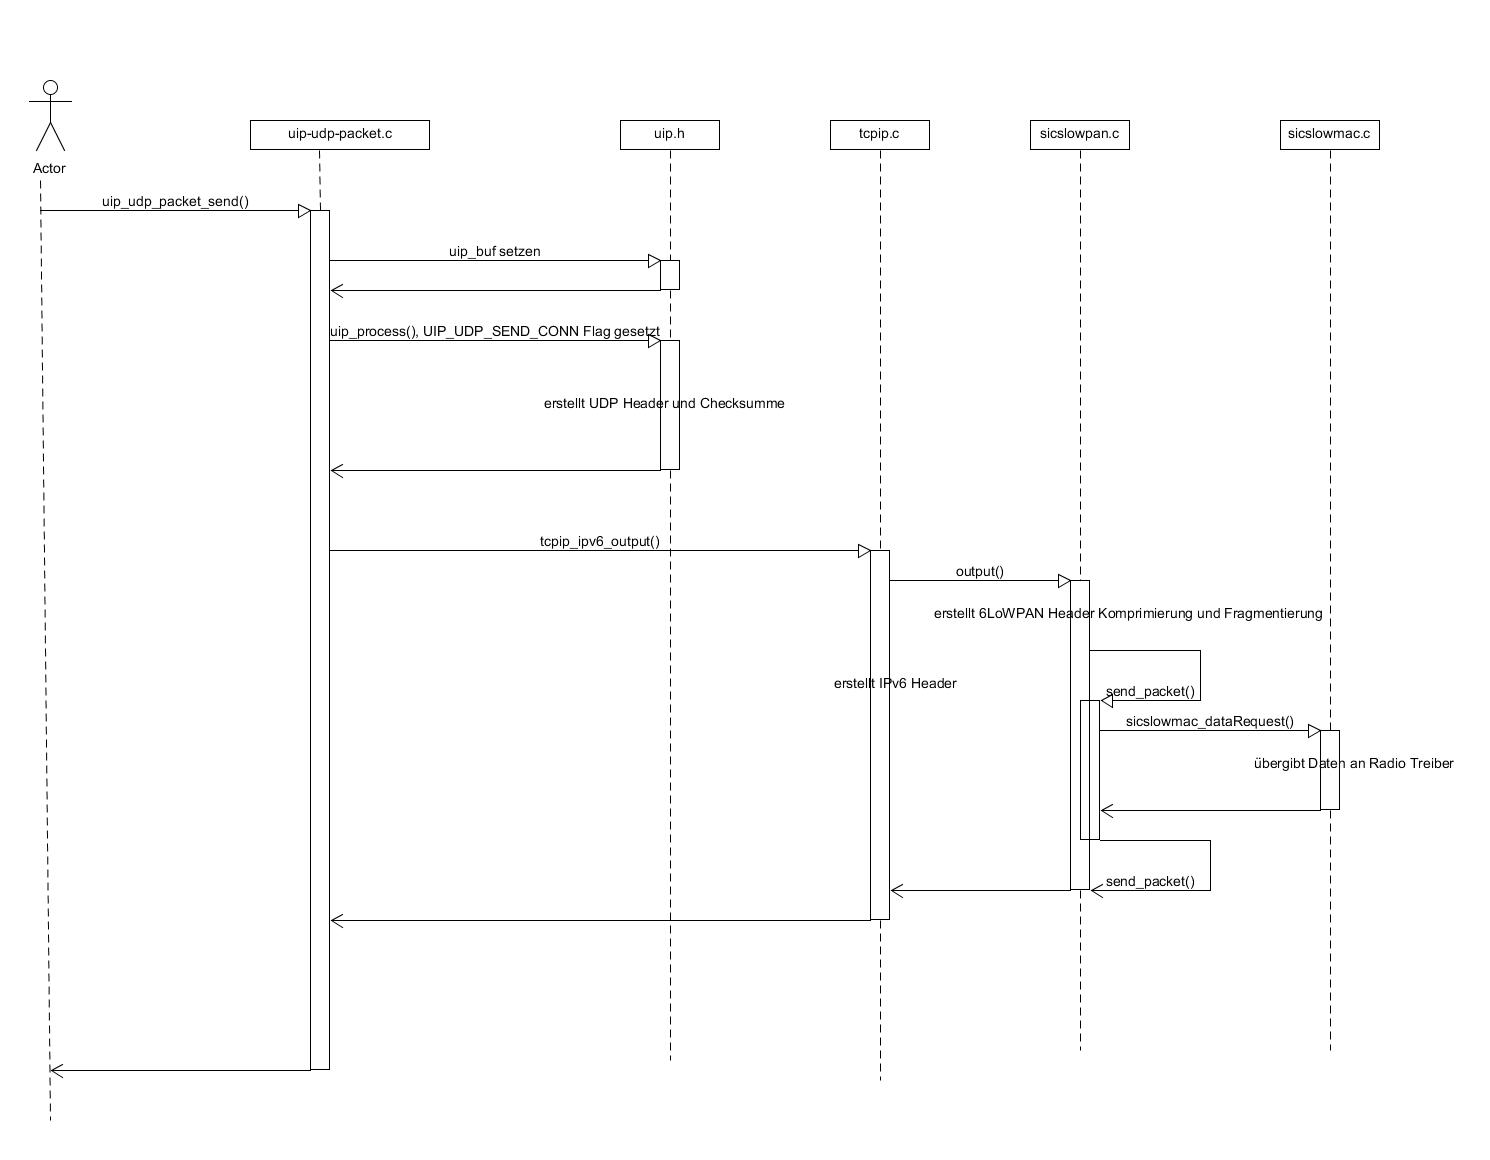
\includegraphics[scale=0.33]{Grafiken-Julian/SendPacket.jpg}
			\caption{Sequenzdiagramm des Funktionsaufruf uip\_udp\_packet\_send() nach nach \cite{sendreceive}}
			\label{SendPacket}
		\end{figure}
		\item Paket empfangen\\
		Abbildung \ref{ReceivePacket} zeigt beispielhaft den Programmablauf bei Empfang eines Pakets. Generell ist der interne Funktionsablauf bei Empfang eines Pakets immer gleich. Wie das Paket weiter verarbeitet wird, entscheidet ein anderer Prozess innerhalb des Ablaufs.\\
		Wird ein Paket empfangen leitet das Funkmodul diese Daten an die sicslowmac\_dataIndication() (siclowmac.c) weiter. Diese Funktion speichert die ankommenden Daten in den Paketbuffer der paketbuf.c Datei. Ist ein Paket komplett empfangen wird mithilfe der Datenlänge der Headerbereich von der Payload mit der Funktion paketbuf\_set\_datalen() getrennt. Anschließen werden die einzelne Fragmente mit der Funktion input() (siclowpan.c) wieder zusammengesetzt und der \ac{ipv6} Header wird wieder dekomprimiert. Im Verlauf dieser Funktion wird dann auch ein synchroner Event an den tcpip\_process() (tcpip.c) ausgelöst. Innerhalb dieser Funktion werden weitere Schritte vorgenommen, um das Paket und die darin enthaltene Payload zu verwerten. Letztendlich wird in der Funktion uip\_process() die zuständige Callback Funktion des Programmierers aufgerufen.\\
		Der gesamte Programmablauf soll Abbildung \ref{ReceivePacket} verdeutlichen.
		\begin{figure}
			\centering
			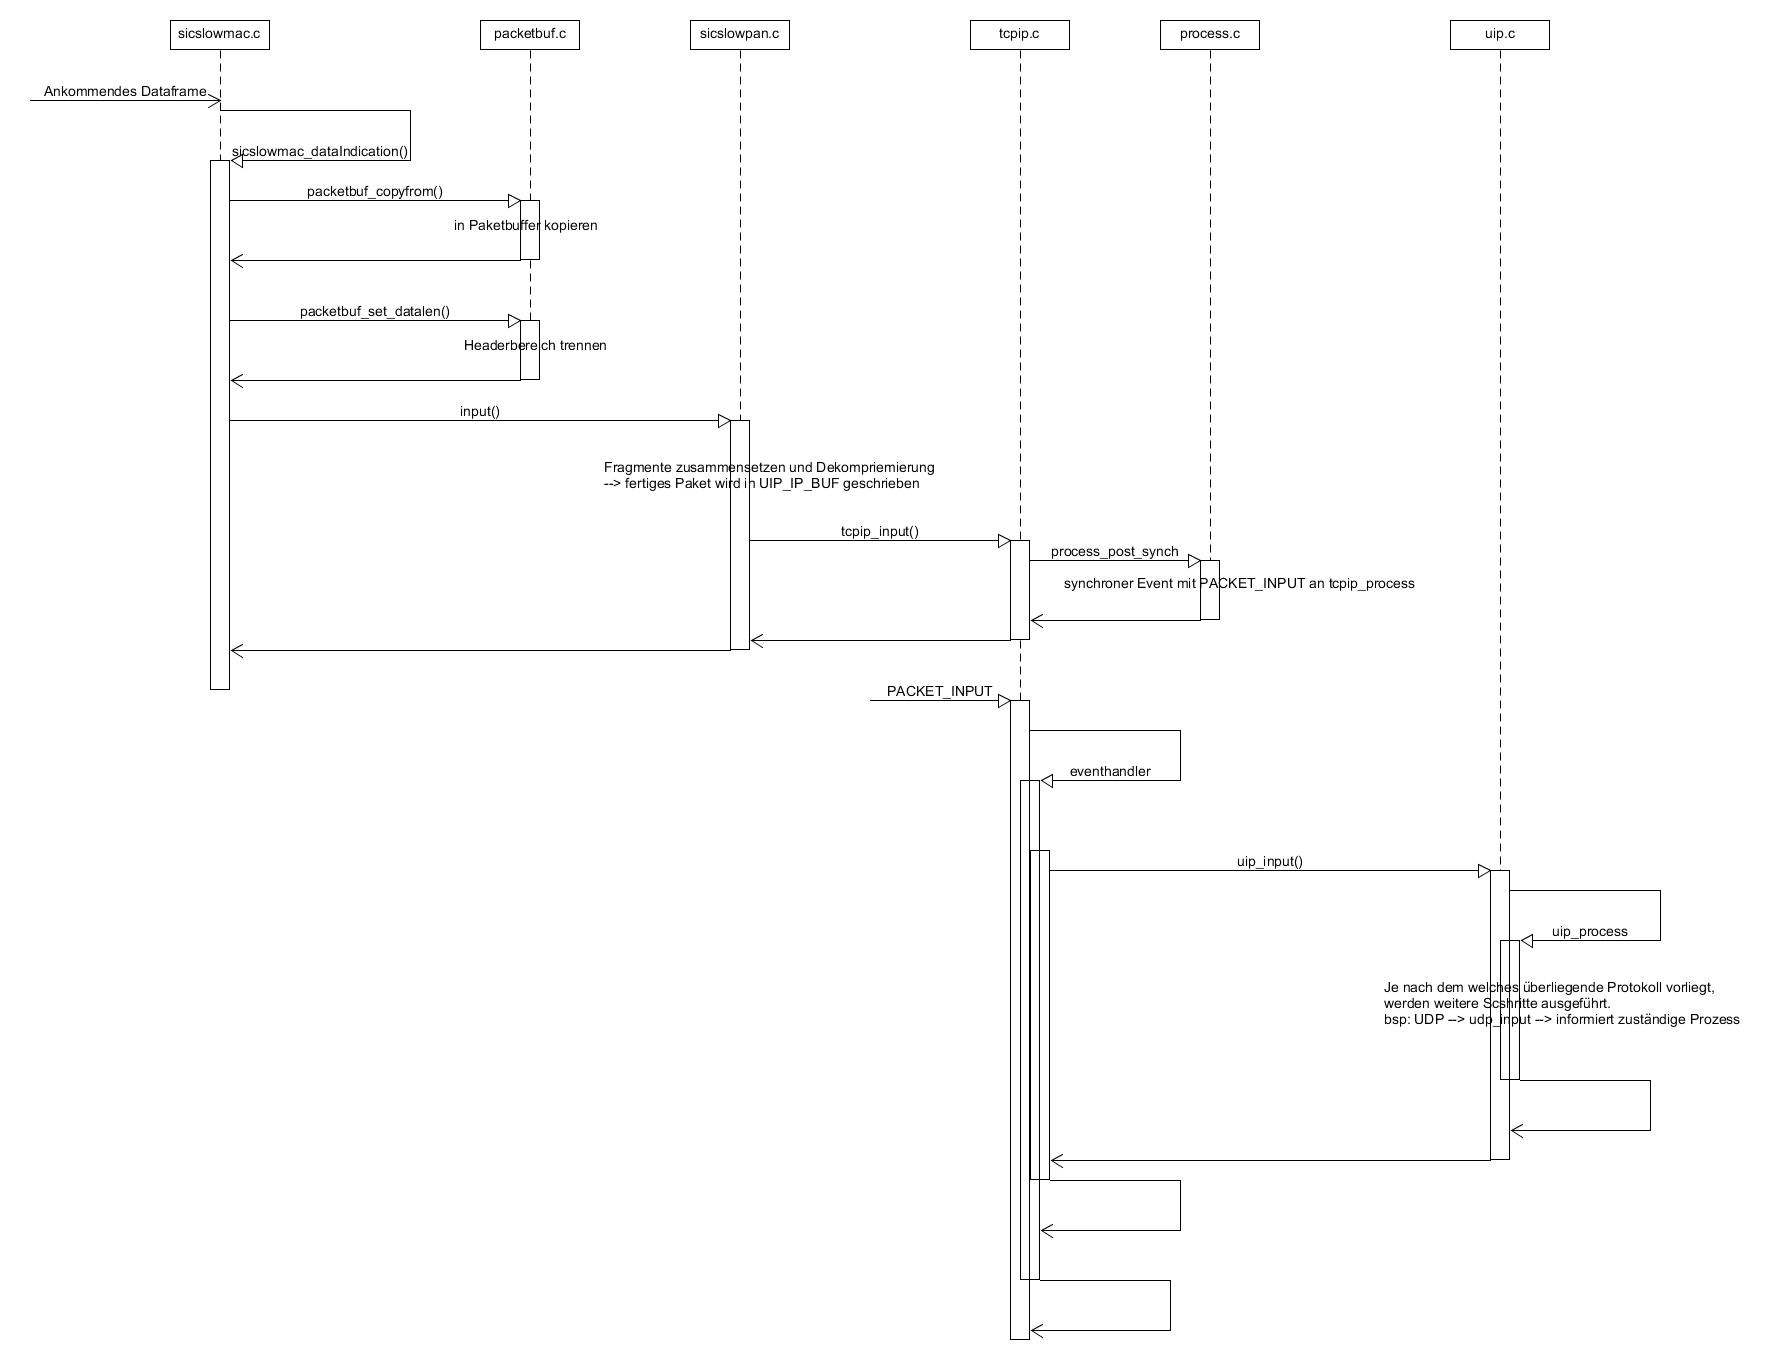
\includegraphics[scale=0.28]{Grafiken-Julian/ReceivePacket.jpg}
			\caption{Sequenzdiagramm bei Empfangen eines Pakets nach \cite{sendreceive}}
			\label{ReceivePacket}
		\end{figure}
		
	\end{itemize}
	
\newpage
\section{Beispielhafte Implementierung eines 6LoWPAN-Netzwerks auf Basis von Contiki}
Um die Implementierung eines 6LoWPAN-Netzwerks mit Contiki beispielhaft darzulegen, haben wir ein Netzwerk bestehend aus mehreren Nodes und einem Edge-Router selbst programmiert. Die Nodes können über eine \ac{uart} Schnittstelle mit dem Nutzer interagieren. Im realen Einsatz wäre zwar eine Machine-to-Machine-Kommunikation wünschenswert, jedoch würde diese zu einem weniger anschaulichen Ergebnis führen. \\
Um die einzelnen Nodes und gegebenenfalls den Edge-Router zu programmieren, haben wir eine kleine Skriptsprache bestehend aus wenigen Befehlen entwickelt. So kann beispielsweise die eigene IP-Adresse abgefragt werden oder es können Pakete mit dem gewünschten Inhalt an Empfänger innerhalb und außerhalb des Netzwerks geschickt werden. \\
Weil die Implementierung eines richtigen Edge-Routers wie er in 6LoWPAN definiert ist den Rahmen dieses Projekts sprengen würde, haben wir uns einer Hilfslösung bedient. Im 6LoWPAN fungiert ein Teilnehmer mit leicht verändertem Code als Ziel für Pakete, die das Netzwerk verlassen sollen. Diese Pakete sind auf der IP-Schicht und UDP-Schicht an eben diesen Teilnehmer adressiert und enthalten die Adressen bzw. den Ports des eigentlichen Empfängers in der Payload. Der Teilnehmer erkennt ein solches Paket und schickt die Nutzdaten, die Quell- und Zieladresse, und den Quell- sowie Zielport über UART an einen anderen Controller. Dieser wiederum generiert aus der UART-Nachricht ein UDP/IP-Paket und schickt es über Ethernet an den Adressaten.\\
Will ein Teilnehmer außerhalb des 6LoWPAN eine Node innerhalb dieses Netzwerks erreichen, so schickt er ein Paket, das auf UDP- und IP-Schicht an den UART-Partner des 6LoWPAN adressiert ist und Zieladresse und Port wiederum nebst eigentlichen Nutzdaten in der Payload enthält. Wieder werden die relevanten Daten über UART ausgetauscht und im 6LoWPAN an den richtigen Empfänger weitergeleitet. Mit wenigen Einschränkungen kann man also das über UART kommunizierende Bündnis in seiner Gesamtheit als Edge-Router betrachten. Abbildung \ref{beispielnetzwerk} zeigt den Aufbau des Projekts anschaulich.\\
\begin{figure}
	\centering
	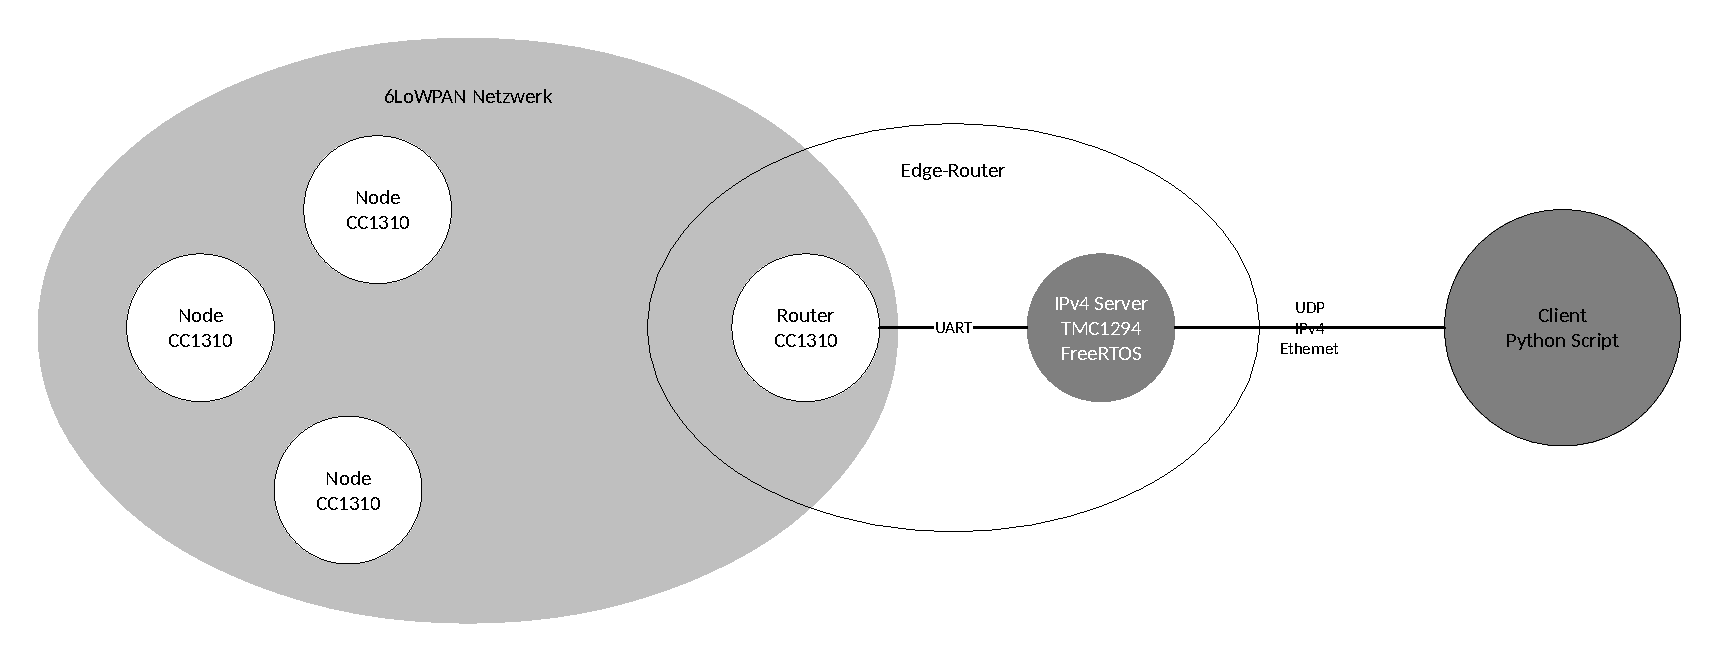
\includegraphics[width=\textwidth]{Grafiken-Alex/beispielnetzwerk.pdf}
	\caption{Der Aufbau unseres Beispielnetzwerks}
	\label{beispielnetzwerk}
\end{figure}

\subsection{Eingesetzte Hardware}
Die einzelnen Nodes bestehen hauptsächlich aus dem CC1310, einem 15.4-fähigen Mikrocontroller von Texas Instruments. Um die Arbeit mit diesem Controller zu vereinfachen, wurden das zugehörige Launchpad verwendet, welches vor allem durch die bereits bestehende Antenne den Entwicklungsaufwand stark reduziert und es uns ermöglichte, uns auf das eigentlich wesentliche Thema zu konzentrieren. \\
Auch der Edge-Router besteht 6LoWPAN-seitig aus einem CC1310 Launchpad. Dieses ist durch eine einfache Jumper-Verbindung, die die UART-Kommunikation ermöglicht mit einem TI129EXL-Launchpad verbunden. Dieses wiederum bietet die Möglichkeit der Kommunikation nach außen durch Ethernet. 

\subsection{Konventionen}
Um ein ordentliches Routing von Paketen durch den Edge-Router zu ermöglichen, mussten gewisse Konventionen ausgearbeitet werden. Diese beinhalten den Aufbau eines Pakets, dessen Source oder Destination außerhalb des 6LoWPAN liegt in der Kommunikation zwischen
\begin{itemize}
	\item Node und Edge-Router über IEEE 802.15.4
	\item CC1310 und TI1294 über UART
\end{itemize}
Es war nicht möglich, hier den gleichen Paketaufbau einzusetzen, weil über UART in den Nutzdaten, Informationen mitgeteilt werden, die über 15.4 schon durch die Header ersichtlich sind - beispielsweise die IPv6-Adresse des 6LoWPAN-seitigen Kommunikationspartners. Die Grafiken \ref{komm-intern} und \ref{komm-extern} zeigen den jeweiligen Aufbau eines Routing-Pakets.

\begin{figure}
	\centering
	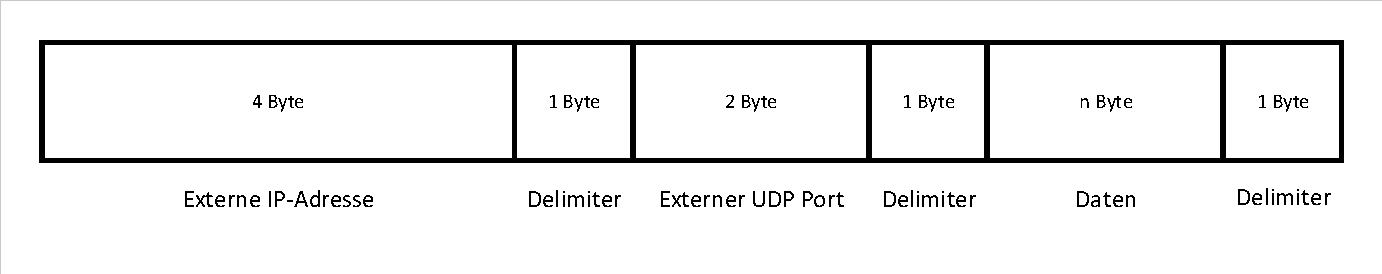
\includegraphics[width=\textwidth]{Grafiken-Alex/komm-intern.pdf}
	\caption{Aufbau eines Routing-Pakets innerhalb des 6LoWPAN. Als Delimiter wird 0x2E (entspricht in ASCII einem Punkt) eingesetzt.}
	\label{komm-intern}
\end{figure}
\begin{figure}
	\centering
	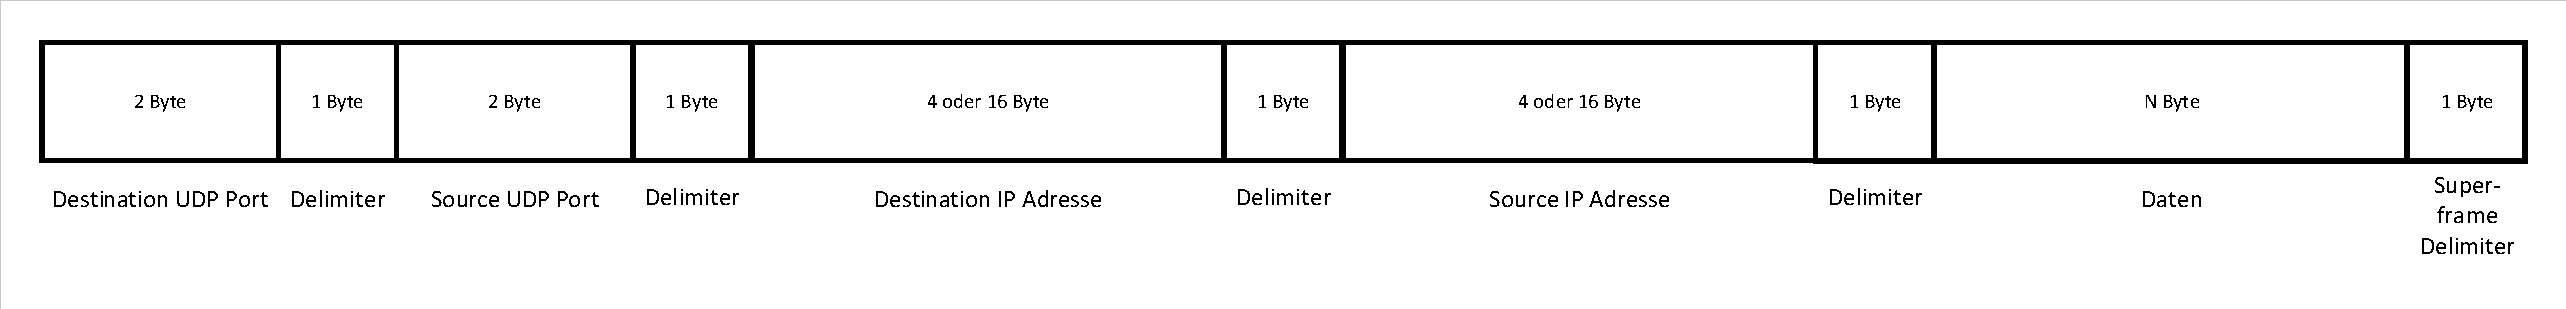
\includegraphics[width=\textwidth]{Grafiken-Alex/komm-extern.pdf}
	\caption{Aufbau eines Routing-Pakets zur UART-Kommunikations. Als Delimiter wird 0x2E (entspricht in ASCII einem Punkt) und als Superframe Delimiter 0x0A (entspricht in ASCII dem New-Line-Character) eingesetzt.}
	\label{komm-intern}
\end{figure}

\subsection{Inbetriebnahme}
Zur Inbetriebnahme muss die Software zunächst kompiliert werden. Zu diesem Zweck bietet sich Instant Contiki an, da es bereits eine funktionierende Toolchain für Contiki mitbringt. Zunächst muss aber die Software noch gemäß den Anforderungen eingestellt werden. Dies geschieht im File configuration.h mit folgenden Defines.
\begin{itemize}
	\item MODE 		
	\item RPLDEVICE	
	\item TARGET		
\end{itemize}
Die Software wurde nicht nur für den tatsächlichen Einsatz, sondern auch zum Debuggen angefertigt. In letzterem Fall werden sämtliche relevante Ereignisse über UART kommentiert. Mit dem Define MODE kann mit den Optionen RELEASE oder DEBUG ausgewählt werden, auf welche Art die Software kompiliert wird. Der Define RPLDEVICE spezifiziert, ob es sich um eine Node oder die Root handelt und kann durch NODE oder ROOT spezifiziert werden. Zu guter Letzt kann bei TARGET für einen bestimmten Prozessor kompiliert werden. Das Target wird zwar auch beim Build Prozess mitgeteilt, aber im Quellcode ändern sich einzelne Kommandos (z.B. der Einsatz des UART Moduls) in Abhängigkeit des verwendeten Targets. Derzeit werden hier die Optionen Z1 (sinnvoll für den Simulator) und CC1310 unterstützt. Beispielsweise könnte die Konfiguration einer Node als Release wie folgt aussehen.\\
\\
\emph{\#define MODE 		RELEASE \\	
	\#define RPLDEVICE	NODE \\	
	\#define TARGET		CC1310 } \\

Zum Kompilieren navigiert man mit der Kommandozeile in den Ordner, an dem das Projekt liegt und gibt den folgenden Build-Command ein: \\
\emph{make TARGET=srf06-cc26xx BOARD=cc1310/launchpad udp-node.bin} \\
Äquivalent dazu lautet der Build-Command für eine Root \\
\emph{make TARGET=srf06-cc26xx BOARD=cc1310/launchpad udp-root.bin} \\
Sollte eine Fehlermeldung, die besagt, dass Contiki nicht gefunden werden konnte, erscheinen, muss im File MAKEFILE in der Zeile \\
\emph{CONTIKI = ../../contiki} \\
der korrekte Pfad zum Ordner von Contiki mitgeteilt werden. Die Standard-Konfiguration funktioniert beispielsweise, wenn der Projektordner auf dem Desktop und Contiki im Home-Folder liegt. Die fertigen Binaries können nun beispielsweise mit dem Flash Programmer 2 geflasht werden. 

\subsection{Übersicht der Befehle zur Steuerung der Teilnehmer}
Für Nodes funktionieren alle Befehle sowohl im DEBUG als auch im RELEASE Modus. Die Root ist im ROOT Modus nicht zur UART-Kommunikation mit Menschen ausgelegt, weshalb hier keine Befehle funktionieren. \\
Da Edge Router und Root die gleiche Firmware benutzen, handelt es sich hier um ein Gerät und beide Begriffe können im Kontext dieses Projekts synonym verwendet werden. \\
\begin{longtable}{l|p{4cm}|p{4cm}|p{2cm}|p{4cm}|p{4cm}}
	\textbf{Kategorie} & \textbf{Befehl} & \textbf{Beschreibung} & \textbf{Gerätetyp} & \textbf{Beispiel} & \textbf{Anmerkung} \\
	\toprule[1.5pt] &&&&&\\
	\textbf{Allgemein} & print id & Zeigt ID von bereitgestelltem Service an. & Node, Root & print id & \\
	\midrule
	& print ip & Zeigt eigene IPv6-Adresse an & Node, Root  & print ip \\
	\midrule
	& hello & Grüßt Teilnehmer und stellt sich vor & Node, Root & hello \\
	& hello device &&&&\\
	\bottomrule[1.5pt] &&&&&\\
	\textbf{Servreg-Hack} & service register [ID] & Stellt Service mit ID [ID] bereit. & Node, Root & service register 150
	& Root registriert im Release automatisch Servive mit ID 190 \\
	\midrule
	& service get ip [ID] & IP von Teilnehmer, der Service mit ID [ID] bereitstellt anzeigen.
	& Node, Root & service get ip 180 \\
	\midrule
	& service edge [ID] & Speichert die ID des Edge Routers. & Node & service edge 190 & Überprüft, ob Root Service mit dieser ID anbietet. \\
	\bottomrule[1.5pt] &&&&&\\
	\textbf{UDP} & udp send id [ID] [DATA] & Sendet Nachricht [DATA] an Teilnehmer mit ID [ID]. & Node, Root & udp send id 190 Hello World! \\
	\midrule
	& udp send ip [IP] [DATA] & Sendet Nachricht [DATA] an Teilnehmer mit IPv6 [IP]. & Node, Root & udp send ip ffd::1 Hello World! & Außer „::“ am Anfang oder Ende und „.“ statt „:“ alle IPv6-Konventionen unterstützt. Es findet keine Überprüfung der eingegebenen IPv6-Adresse statt! \\
	\midrule
	& udp send extern [IP] [PORT] [DATA] & Sendet UDP an Edge-Router, der die Nachricht [DATA] an Teilnehmer mit IPv4 [IP] und Port [PORT] weiterleitet. & Node & udp send extern 192.168.200.99 5005 Hello World! & ID des Edge Routers muss bekannt sein. Zuvor per \emph{service edge [ID]} bereitstellen. \\
	\bottomrule[1.5pt]
	
	
	
	
	
\end{longtable}
\newpage
\section*{Abkürzungsverzeichnis}
\begin{acronym}[6LoWPAN]
	\acro{15.4}[15.4]{IEEE 802.15.4}
	\acro{6lowpan}[6LoWPAN]{IPv6 over Low power Wireless Personal Area Network}
	\acro{bpsk}[BPSK]{Binary Phase Shift Keying}
	\acro{caa}[CCA]{Clear Channel Assessment}
	\acro{cap}[CAP]{Contention Access Period}
	\acro{cfp}[CFP]{Collision Free Period}
	\acro{crc}[CRC]{Cyclic Redundancy Check}
	\acro{csmaca}[CSMA/CA]{Carrier Sense Multiple Acces with Collision Avoidance}
	\acro{csmacd}[CSMA/CD]{Carrier Sense Multiple Acces with Collision Detection}
	\acro{dsss}[DSSS]{Direct Sequence Spread Spectrum}
	\acro{eui64}[EUI-64]{64-Bit Extended Unique Identifier}
	\acro{fcs}[FCS]{Frame Check Sequence}
	\acro{ffd}[FFD]{Full-Function Device}
	\acro{gts}[GTS]{Guaranteed Time Slot}
	\acro{ieee}[IEEE]{Institute of Electrical and Electronics Engineers}
	\acro{iot}[IoT]{Internet of Things}
	\acro{ip}[IP]{Internet Protocol}
	\acro{ipv4}[IPv4]{Internet Protocol Version 4}
	\acro{ipv6}[IPv6]{Internet Protocol Version 6}
	\acro{k}[k]{kilo}
	\acro{llc}[LLC]{Logical Link Control}
	\acro{m}[m]{milli}
	\acro{mac}[MAC]{Medium Access Control}
	\acro{mpdu}[MPDU]{MAC Protocol Data Unit}
	\acro{msdu}[MSDU]{MAC Service Data Unit}
	\acro{mtu}[MTU]{Maximum Transmission Unit}
	\acro{nrz}[NRZ]{Non-return to zero}
	\acro{oqpsk}[O-QPSK]{Offset Quadrature Phase Shift Keying}
	\acro{osi}[OSI]{Open System Interconnection}
	\acro{pan}[PAN]{Personal Area Network}
	\acro{pc}[PC]{Personal Computer}
	\acro{phy}[PHY]{Physical}
	\acro{ppdu}[PPDU]{PHY Protocol Data Unit}
	\acro{psdu}[PSDU]{PHY Service Data Unit}
	\acro{pdu}[PDU]{Protocol Data Unit}
	\acro{qam}[QAM]{Quadraturamplitudenmodulation}
	\acro{rfd}[RFD]{Reduced-Function Device}
	\acro{sdu}[SDU]{Service Data Unit}
	\acro{sics}[SICS]{Swedish Institute of Computer Science}
	\acro{soc}[SoC]{System on a Chip}
	\acro{tcp}[TCP]{Transmission Control Protocol}
	\acro{uart}[UART]{Universal Asynchronous Receiver and Transmitter}
	\acro{udp}[UDP]{User Datagram Protocol}
	\acro{w}[W]{Watt}
	\acro{wpan}[WPAN]{Wireless Personal Area Network}
	\acro{www}[WWW]{World Wide Web}
\end{acronym}
\newpage
\bibliographystyle{plaindin}
\bibliography{sources}


\end{document}